\documentclass[12pt,a4paper]{report}

\usepackage[utf8]{inputenc} % pentru suport diacritice
\usepackage[english]{babel} % setări pentru limba română 
\renewcommand\familydefault{\sfdefault} % sans serif

\usepackage[margin=2.54cm]{geometry}	% dimensiuni pagină și margini
\usepackage{graphicx} % support the \includegraphics command and options

% formatting sections and subsections
\usepackage{float}
\usepackage{textcase}
\usepackage[titletoc, title]{appendix}
\usepackage{titlesec}
\titleformat{\chapter}{\large\bfseries\MakeUppercase}{\thechapter}{2ex}{}[\vspace*{-1.5cm}]
\titleformat*{\section}{\large\bfseries}
\titleformat*{\subsection}{\large\bfseries}
\titleformat*{\subsubsection}{\large\bfseries}

\usepackage{chngcntr}
\counterwithout{figure}{chapter} % no chapter number in figure labels
\counterwithout{table}{chapter} % no chapter number in table labels
\counterwithout{equation}{chapter} % no chapter number in equation labels

\usepackage{booktabs} % for much better looking tables
\usepackage{xcolor}
\usepackage{listings}
\usepackage{url} % Useful for inserting web links nicely
\usepackage[bookmarks,unicode,hidelinks]{hyperref}

\usepackage{array} % for better arrays (eg matrices) in maths
\usepackage{amsmath} % extended mathematical notation
\usepackage{paralist} % very flexible & customisable lists (eg. enumerate/itemize, etc.)
\usepackage{verbatim} % adds environment for commenting out blocks of text & for better verbatim
\usepackage{subfig} % make it possible to include more than one captioned figure/table in a single float
\usepackage{enumitem}
\setlist{noitemsep}

\lstdefinestyle{annexcode}{
  basicstyle=\ttfamily\tiny,
  backgroundcolor=\color{gray!8},
  frame=single,
  rulecolor=\color{gray!45},
  breaklines=true,
  breakatwhitespace=false,
  columns=fullflexible,
  keepspaces=true,
  showstringspaces=false,
  tabsize=2,
  aboveskip=0.5em,
  belowskip=0.8em,
  xleftmargin=0.5em,
  xrightmargin=0.5em
}

%%% HEADERS & FOOTERS
\usepackage{fancyhdr}
\pagestyle{empty}
\renewcommand{\headrulewidth}{0pt}
\renewcommand{\footrulewidth}{0pt}
\lhead{}\chead{}\rhead{}
\lfoot{}\cfoot{\thepage}\rfoot{}



\newcommand{\HeaderLineSpace}{-0.25cm}
\newcommand{\UniTextRO}{UNIVERSITATEA POLITEHNICA DIN BUCUREȘTI \\[\HeaderLineSpace] 
FACULTATEA DE AUTOMATICĂ ȘI CALCULATOARE \\[\HeaderLineSpace]
DEPARTAMENTUL DE CALCULATOARE\\}
\newcommand{\DiplomaRO}{PROIECT DE DIPLOMĂ}
\newcommand{\AdvisorRO}{Coordonator științific:}
\newcommand{\BucRO}{BUCUREȘTI}

\newcommand{\UniTextEN}{UNIVERSITY POLITEHNICA OF BUCHAREST \\[\HeaderLineSpace]
FACULTY OF AUTOMATIC CONTROL AND COMPUTERS \\[\HeaderLineSpace]
COMPUTER SCIENCE AND ENGINEERING DEPARTMENT\\}
\newcommand{\DiplomaEN}{SEMESTRIAL REPORT}
\newcommand{\AdvisorEN}{Thesis advisor:}
\newcommand{\BucEN}{BUCHAREST}

\newcommand{\frontPage}[6]{
\begin{titlepage}
\begin{center}
{\Large #1}  % header (university, faculty, department)
\vspace{50pt}
\begin{tabular}{p{6cm}p{4cm}}

\end{tabular}

\vspace{105pt}
{\Huge #2}\\                           % diploma project text
\vspace{40pt}
{\Large #3}\\ \vspace{0pt}  % project title
{\Large #4}\\                          % project subtitle
\vspace{40pt}
{\LARGE \Name}\\                   % student name
\end{center}
\vspace{60pt}
\begin{tabular*}{\textwidth}{@{\extracolsep{\fill}}p{6cm}r}
&{\large\textbf{#5}}\vspace{10pt}\\      % scientific advisor
&{\large \Advisor}                                    % advisor name
\end{tabular*}
\vspace{20pt}
\begin{center}
{\large\textbf{#6}}\\                                % bucharest
\vspace{0pt}
{\normalsize \Year}
\end{center}
\end{titlepage}
}

\newcommand{\frontPageEN}{\frontPage{\UniTextEN}{\DiplomaEN}{\ProjectTitleEN}{\ProjectSubtitleEN}{\AdvisorEN}{\BucEN}}

\linespread{1.15}
\setlength\parindent{0pt}
\setlength\parskip{.28cm}

%% Abstract macro
\newcommand{\AbstractPage}{
\begin{titlepage}
\textbf{\large ABSTRACT}\par
\AbstractEN \vfill
\end{titlepage}
}



%%%%%%%%%%%%%%%%%%%%%%%%%%%%%%%%%%%%%%%%%%%%%%%%%%   
%%
%%          End of template definitions
%%   
%%%%%%%%%%%%%%%%%%%%%%%%%%%%%%%%%%%%%%%%%%%%%%%%%%


%%% Puteți elimina aceste linii din lucrare, servesc numai pentru template.
\newcommand{\worktype}[1]{[\textit{#1}] }
\newcommand{\dezvoltare}{\worktype{Dezvoltare de produs}}
\newcommand{\cercetare}{\worktype{Cercetare}}
\newcommand{\ambele}{\worktype{Ambele}}
%%%


%%
%%   Campurile de mai jos trebuie modificate de autor. Modificati doar continutul, nu si numele fiecarei definitii
%%
\newcommand{\ProjectTitleRO}{Infrastructură ROS automatizată}
\newcommand{\ProjectSubtitleRO}{Orchestrare prin șabloane ghidată de modele lingvistice}
\newcommand{\ProjectTitleEN}{Automated ROS Infrastructure}
\newcommand{\ProjectSubtitleEN}{Orchestration via LLM-Driven Templating}
\newcommand{\Name}{Alfred Andrei Pietraru}
\newcommand{\Advisor}{Prof. dr. ing. Dan Marius Novischi}
\newcommand{\Year}{2026}

% Setări document
\title{Proiect de diplomă}
\author{\Name}
\date{\Year}

%%
%%   Campurile aferente rezumatului
%%
\newcommand{\AbstractEN}{Modern robotic platforms such as the AntRobot operate within complex software ecosystems based on the Robot Operating System (ROS2) \cite{quigley2009ros} \cite{macenski2022ros2} where system functionality is distributed across multiple interconnected nodes responsible for perception, localization, mapping, planning, and control. Although ROS promotes modular design, configuring these nodes remains a largely manual and error-prone process. Even minor changes, such as switching sensors, modifying mission modes, or adjusting parameters, often require extensive manual edits across multiple YAML and launch files.

This repetitive configuration effort limits reproducibility, scalability, and experimentation speed in both research and applied robotics. Existing orchestration solutions, including ROScribe and RobotKube, provide partial automation but continue to rely on static configuration schemes that restrict flexibility and reuse.

This work proposes a hybrid ROS orchestration framework that combines source-grounded repository analysis, bounded language-model reasoning, and deterministic configuration generation. Static analysis extracts ROS~2 nodes, launch structure, parameters, interfaces, and provenance into a versioned system model. A large language model (LLM) interprets high-level mission descriptions, selects parameters only from retrieved evidence, and proposes typed values. Strict schemas and deterministic checks validate these conclusions before Jinja2 templates materialize launch and YAML artifacts; the model never writes ROS files directly.

The prototype derives 109 writable configuration slots from the AntRobot workspace and was evaluated on 150 generated mission paraphrases grouped around 15 verified intents, together with a five-case diagnostic set. The initial local-model baseline achieved 76.1\% capability micro $F_1$, but only 1.6\% parameter-selection micro $F_1$ and no jointly exact missions. Few-shot prompting improved supported-outcome accuracy and partial parameter recovery, but did not improve exact end-to-end correctness. These results demonstrate both the feasibility of the hybrid architecture and the importance of grounded retrieval, constrained parameter identification, independent human review, and boundary-specific evaluation.}

\begin{document}

\frontPageEN

\begingroup
\linespread{1}
\setlength{\parskip}{0pt}
\tableofcontents
\endgroup

\AbstractPage{}

% \chapter{Introduction}\pagestyle{fancy}
ROS-based robotic systems are constructed from loosely coupled nodes that communicate via a publisher–subscriber architecture. Each node typically performs a well-defined task, such as sensor data acquisition, state estimation, or motion planning. Although this separation of concerns promotes modularity, it also requires careful coordination of parameters, topic names, frame hierarchies, and execution dependencies.

Recent developments in cloud robotics, containerization, and orchestration frameworks have improved deployment scalability. Tools such as RobotKube \cite{lampe2023robotkube} and FogROS \cite{fogros22023} facilitate distributed execution and infrastructure management. Meanwhile, language-based systems such as ROScribe \cite{roscribe} demonstrate the feasibility of using large language models (LLMs) to generate code and launch structures from natural language instructions. However, existing approaches either focus primarily on infrastructure orchestration or code generation, and they typically lack a structured reasoning layer capable of translating high-level mission intent into coherent configuration artifacts.

At the same time, LLMs have shown strong capabilities in structured output generation, including JSON schema adherence and code synthesis. This creates an opportunity to explore their integration into robotic configuration pipelines while preserving determinism and structural validity in downstream system assembly.

Despite the modular architecture of ROS, configuring a robotic system remains a highly manual and error-prone process. Small changes in mission objectives—such as switching sensors, enabling mapping, or modifying operational modes—often require updates across multiple YAML files and launch scripts. These modifications must remain internally consistent, particularly with respect to frame identifiers, topic mappings, and dependency relationships between nodes.
Current orchestration tools do not provide a unified mechanism to transform high-level semantic descriptions of robotic tasks into fully consistent ROS deployments. As a result, robotic system configuration 
remains tightly coupled to domain expertise and manual engineering 
effort. The absence of a structured pipeline connecting mission intent
to executable configuration limits reproducibility, slows 
experimentation, and increases the likelihood of integration errors. The problem addressed in this work is how can natural-language mission
descriptions be systematically translated into valid, coherent, and executable
ROS configurations in a deterministic and reproducible manner.
% \chapter{Problem Analysis}
\section{ROS-Based Robotic Systems Overview}
Nowadays robotic systems are increasingly built as distributed software architectures composed of multiple interacting components.
The Robot Operating System (ROS) has become the standard framework when developing such systems, providing a flexible middleware
that enables modularity, reuse, and interoperability across heterogeneous hardware and software platforms. In ROS-based systems,
functionality is decomposed into nodes, each responsible of a well-defined task. These nodes communicate through message passing mechanisms using topics, services, and actions, forming a 
dynamic computation graph. This publisher-subscriber architecture enables developers to construct complex robotic behaviors. Nodes can be developed independently, deployed on different machines, and connected at runtime,
allowing robotic systems to scale from single embedded devices to distributed setups.

Additionally, ROS supports a wide ecosystem of third-party packages that implement common algorithms and hardware interfaces,
significantly reducing development effort. However, the flexibility offered by ROS also introduces complexity. The overall system
behavior emerges not only from the implementation of individual nodes, but also from how they are connected, configured, and parameterized.
The ROS computation graph may involve dozens of nodes with intricate dependencies on sensors, coordinate frames, timing assumptions, and
runtime parameters. As a result, the correctness and performance of the system depend heavily on the configuration choices made during deployment.
More than that, ROS itself intentionally avoids imposing strong constraints on how systems should be structured. While this design choice promotes
generality and reusability, it places a significant burden on developers to ensure that node interactions are valid for a given task.

As robotic systems grow in scale and complexity, understanding and managing these interactions becomes challenging,
particularly when systems must be adapted to new missions, hardware configurations, or operational environments. 
Beyond software modularity, ROS-based systems must also operate under real-world constraints that further complicate system design. Robotic
applications are often required to integrate heterogeneous sensors, operate under strict timing requirements, and interact with uncertain
and dynamic environments. These constraints introduce implicit assumptions into system configurations, such as expected sensor frequencies,
coordinate frame hierarchies, and synchronization between perception and control pipelines. While ROS provides the communication primitives
needed to express these interactions, it does not enforce correctness or consistency at the system level. As a result, many design decisions 
are encoded implicitly in configuration files rather than being explicitly represented or validated. This implicit knowledge becomes increasingly
difficult to maintain as systems evolve, particularly when configurations are reused across different platforms or mission scenarios.

\section{ROS Configuration and Orchestration Challenges}
Configuring a ROS-based robotic system involves more than launching executable nodes. Developers must specify a wide range of parameters that govern
node behavior, communication interfaces, sensor usage, and algorithmic settings. These configurations are typically expressed through a combination 
of launch files, parameter files, often in YAML format, and environment-specific settings. Even minor changes, such as replacing a sensor or adjusting
an algorithm parameter, may require coordinated updates across multiple configuration files. Orchestration further complicates this process. In 
distributed deployments, nodes may be executed across multiple machines or containers, requiring careful management of networking, synchronization, 
and lifecycle events. Ensuring that nodes are launched in the correct order, recover gracefully from failures, and remain consistent across restarts 
is non-trivial, particularly when systems are deployed in dynamic or resource-constrained environments. 

Existing orchestration mechanisms within ROS provide only limited support for these challenges. Launch files primarily describe static execution
graphs and offer minimal capabilities for conditional logic or dynamic adaptation. External orchestration frameworks, such as container-based 
deployment platforms, can manage process lifecycles and resource allocation but operate largely independently of ROS-specific semantics and in most 
cases such system are not designed and do not support ROS components. As a result, developers must manually bridge the gap between system-level
orchestration and ROS-level configuration. Another key challenge lies in the lack of abstraction over mission intent. ROS configurations describe 
how components are connected and parameterized, but not why a particular configuration is appropriate for a given task. Mission objectives, such as 
exploration, mapping, or navigation are implicitly encoded in configuration choices rather than explicitly represented. This makes it difficult to
reason about configurations at a higher level or to systematically adapt systems to new tasks without extensive manual intervention.

\section{Limitations of Manual and Static Approaches}
The predominant approach to configuring ROS-based systems remains manual and largely static. Developers typically create configuration files by hand,
relying on experience, documentation, and trial-and-error to achieve correct system behavior. While this approach may be manageable for small systems 
or fixed use cases, it does not scale well as systems grow in complexity or must support multiple operational modes. Manual configuration is inherently
error-prone. Parameter mismatches, incompatible topic connections, or incorrect assumptions about sensor availability can lead to subtle runtime 
failures that are difficult to diagnose. Moreover, configurations are often tightly coupled to specific hardware setups and mission contexts, reducing
their reusability across different scenarios. Adapting an existing system to a new task frequently involves duplicating and modifying large portions 
of configuration code, increasing maintenance effort and the risk of inconsistencies. Static configurations also limit adaptability. Once a system is
launched, its structure and parameters typically remain fixed, even if environmental conditions or task requirements change. While dynamic 
reconfiguration mechanisms exist, they are rarely used systematically due to their complexity and lack of integration with higher-level reasoning.
As a result, robotic systems often lack the ability to adjust their behavior automatically in response to changing mission objectives. These limitations
show a fundamental gap between the low-level configuration mechanisms provided by ROS and the high-level reasoning required for flexible, 
mission-driven robotic systems. Closing this gap requires methods that can reason about system structure, parameters, and dependencies in a 
more abstract manner, while still producing concrete, executable configurations.

The lack of standardized abstraction mechanisms further increases orchestration challenges in ROS-based systems. Configuration files often mix 
concerns related to hardware setup, algorithm selection, and mission-specific behavior, resulting in tightly coupled specifications that are 
difficult to reason about independently. While parameter servers and launch-time arguments provide some degree of flexibility, they do not offer
a systematic way to capture higher-level relationships between components. Consequently, orchestration logic is frequently implemented through ad-hoc
scripts or duplicated configuration fragments, making systems harder to extend and validate. This fragmentation also affects reproducibility, as small,
undocumented changes in configuration can significantly alter system behavior without being reflected in versioned source code. 

Another flaw is that understanding the impact of a single parameter change often requires detailed knowledge of multiple interacting components, as well as their 
underlying assumptions. This makes configuration tasks difficult to delegate or automate and limits the ability of non-expert users to deploy or 
modify robotic systems safely. Moreover, the absence of explicit validation or reasoning mechanisms means that many configuration errors are only 
discovered at runtime, potentially leading to system downtime or unsafe behavior. These factors underscore the need for approaches that can externalize
configuration knowledge, reduce manual effort, and support systematic reasoning about system structure and behavior.
% \chapter{State of the Art and Related Work}

\section{Existing Orchestration Frameworks}
ROS creates a separation of concerns by using nodes that execute clearly defined tasks and communicate with one 
another through message passing by implementing a publisher subscriber architecture. In a ROS system, nodes communicate
extensively with one another, but they can be abstracted as microservices that are responsible for executing specific 
actions. These microservices usually interact in complex ways that are difficult to handle manually; for this reason, 
technologies such as Kubernetes \cite{verma2015borg} simplify the orchestration of such systems by managing their lifecycles, scaling applications,
and handling errors, thereby creating a fault-tolerant and dynamic system. Although Kubernetes is heavily used in the software domain, it lacks orchestration mechanisms tailored to domains such
as robotics, as it cannot handle ROS-specific concepts such as node graphs, topic compatibility, or sensor algorithm relationships.
RobotKube can improve deployment portability by defining software components that can be containerized using Docker \cite{merkel2014docker} and orchestrated
by Kubernetes, and it can assist with managing the lifecycle of ROS nodes. On the other hand, RobotKube cannot provide mission-driven
orchestration, as the tool has no inherent understanding of the system\'s purpose. Orchestration is achieved through interoperability
with Kubernetes, while the services handled by RobotKube are built using the ROS framework. RobotKube defines robot specific 
resources such as ROS components and initializes the RobotKube Operator which is a controller program. The Operator reacts to 
changes to ROS components and depending on the situation, it can deploy containers, set up networking or restarts components
which previously failed.

ROScribe \cite{roscribe} uses natural language processing to describe system functionalities and generates the initial ROS graph, 
source code, and launch files. ROScribe builds an entire ROS workspace using four agents that are invoked in a sequential order.
First, the SpecAgent constructs the ROS graph of the project by interpreting user requirements and creates a corresponding
development plan. Second, the GenAgent generates the workspace by either retrieving code from public repositories or 
generating code for the required nodes. Third, the PackAgent analyzes the overall workflow and creates the ROS launch 
files, along with additional support files such as package.xml, CMakeLists.txt, and README.md. In some cases, the generated
ROS workspace may contain errors; in this situation, the SupportAgent is responsible for resolving these issues and ensuring
that the system passes static analysis checks. ROScribe automates code writing, launch file generation, and static code analysis
as part of an offline workspace synthesis process. Its operation is limited to the design phase, generating an initial ROS 
workspace based on user descriptions, without adapting configurations at runtime. Also, ROScribe does not handle
parameter configuration, forcing users to manually create and populate the YAML files associated with each node. This 
limitation is significant in ROS-based systems, where parameters are often tightly coupled to sensors, algorithms, and 
mission requirements, making manual configuration repetitive and error-prone. As a result, ROScribe cannot infer or adapt
configurations based on high-level mission intent, relying instead on static, user-defined parameter settings.

FogROS \cite{fogros22023} is an adaptive framework designed to automate the deployment of fog robotics applications. As robotic algorithms become
increasingly complex, particularly in areas such as perception and mapping, edge-based systems may struggle to handle the 
associated computational load under certain conditions. One approach to addressing this limitation is to leverage cloud 
resources, which can provide scalable computational capabilities for demanding operations, subject to network and latency
constraints. FogROS builds on top of the ROS framework and allows users to specify which components of a ROS computation
graph should be executed on cloud resources. FogROS does not provide reasoning or decision-making capabilities, and all 
deployment configurations must be specified manually by the user. As a result, the system cannot infer mission intent or
dynamically adapt configurations based on high-level task descriptions. An additional feature of FogROS is its ability to
automate container creation for cloud deployment, significantly reducing manual setup effort. The framework also supports
flexible networking and pre-deployed nodes, abstracting many aspects of deployment across local devices and cloud environments,
while still requiring user-defined configuration choices.

OSRF Nexus \cite{osrfnexus} is a framework designed to support dependency management and version control within 
ROS-based software ecosystems. It provides mechanisms for organizing, distributing, and resolving
ROS packages and their dependencies across different systems, helping ensure consistency and 
reproducibility of software environments. Nexus operates at the package and dependency level, allowing
developers to manage compatible versions of ROS components without directly modifying application
logic. However, OSRF Nexus focuses exclusively on software dependency resolution 
and does not address system-level configuration or orchestration. It does not generate ROS graphs,
launch files, or parameter configurations, nor does it provide mechanisms for adapting configurations
based on task requirements or mission context. As a result, while Nexus simplifies dependency management
and improves build-time reproducibility, it does not contribute to mission-driven orchestration or 
dynamic configuration synthesis, relying instead on static, user-defined system setups.

Existing tools for ROS-based system development address specific aspects of configuration, 
deployment, or dependency management, but remain limited when considered from a mission-driven
orchestration perspective. ROScribe automates the generation of ROS workspaces, code, and launch 
files at design time, yet produces static artifacts and requires manual parameter configuration, 
lacking support for runtime adaptation or mission-level reasoning. RobotKube improves deployment 
portability and lifecycle management through Kubernetes integration, but relies on pre-defined 
configurations and operates solely at the infrastructure level, without semantic understanding 
of robotic tasks. FogROS focuses on deployment-time placement of ROS nodes across edge and cloud 
resources, assuming pre-existing applications and static configurations, and does not support 
graph synthesis or dynamic reconfiguration. OSRF Nexus enhances dependency and version management,
but does not address configuration generation, orchestration, or task-aware system behavior.

Overall, these approaches improve isolated stages of the ROS workflow while relying on static, 
user-defined configurations. None provide a reasoning layer capable of translating high-level mission
intent into adaptive ROS configurations, highlighting a gap that motivates the proposed research approach.

\begin{table}[H]
\centering
\caption{Comparison of Existing ROS-Oriented Tools}
\label{tab:ros_tools_comparison}
\renewcommand{\arraystretch}{1.3}
\begin{tabular}{|p{3cm}|p{5.5cm}|p{5.5cm}|}
\hline
\textbf{Tool} & \textbf{Provided Capabilities} & \textbf{Limitations} \\
\hline

ROScribe &
Natural-language-driven generation of ROS workspaces, including source code, ROS graphs, launch files, and basic static analysis using a multi-agent pipeline. &
Operates only at design time; generates static artifacts; does not handle parameter configuration, runtime adaptation, or mission-level reasoning. \\
\hline

RobotKube &
Containerized deployment and lifecycle management of ROS-based components using Kubernetes; improves portability, scalability, and infrastructure-level fault tolerance. &
Relies on pre-defined configurations; lacks semantic understanding of ROS graphs, sensor--algorithm relationships, and mission-driven orchestration. \\
\hline

FogROS &
Deployment-time placement of ROS nodes across edge and cloud resources; automated container creation and infrastructure abstraction for fog robotics applications. &
Assumes pre-existing ROS applications and static configurations; does not support graph synthesis, parameter abstraction, or runtime mission adaptation. \\
\hline

OSRF Nexus &
Dependency and version management for ROS packages; improves reproducibility and consistency of ROS software environments. &
Operates solely at the package and dependency level; does not address configuration generation, orchestration, or task-aware system behavior. \\
\hline

\end{tabular}
\end{table}

\section{Language-Based and AI-Driven Robotics Interfaces}
Despite the fact that the outputs of large language models (LLMs) remain nondeterministic, they can still
be integrated into robotic systems in a controlled manner. One example of such integration is ROScribe, 
which leverages LLM-based workflows to automate the generation of ROS workspaces. Similar to the approach 
described in the AutoGen \cite{wu2023autogen} framework, ROScribe employs a multi-agent pipeline in which agents exchange intermediate
artifacts—such as generated code—and invoke external tools to enrich, validate, or evaluate the produced content.
Another relevant work for the current context \cite{ahn2022saycan} demonstrates how high-level task intent
can be extracted from a single natural language instruction and decomposed into multiple subtasks. In this approach, the 
language model proposes candidate actions expressed in natural language, while the robot provides perception and actuation 
capabilities, effectively serving as the interface to the physical environment. The robot is equipped with a set of predefined 
elementary skills, typically involving both perception and motion, which can be composed to execute more complex tasks.
In this framework, the LLM is used to evaluate the suitability of available skills at each step by estimating their contribution 
to task completion through an affordance-based scoring mechanism. The task is defined using a natural language instruction, 
while each elementary skill is associated with a short description and execution constraints. A similar abstraction could be 
applied to ROS-based systems, where nodes are treated as modular components characterized by their code, parameters, dependencies,
and functional descriptions. By maintaining a database of such components, an LLM could identify suitable building blocks and decompose
a high-level task into lower-level configuration requirements, enabling the mapping of individual components to each subtask.
While these approaches focus on task execution and skill selection, they do not address system-level configuration synthesis, 
which remains the focus of the proposed work.

Large language models have consistently demonstrated the ability to generate and adhere to structured output formats such as JSON \cite{thinkinsidejson2025},
which is a crucial requirement for integrating LLMs into software systems. When developing applications that rely on automated 
reasoning, it is often necessary to convert unstructured inputs, such as natural language descriptions, into a fixed set of 
structured representations that can be programmatically processed. In this context, LLMs do not act as code executors, but rather 
as planners and selectors that identify the appropriate tools, components, or configuration options required to fulfill a given task.
This capability is particularly relevant for configuration synthesis tasks,
where downstream systems depend on well-defined and machine-readable representations, such as parameter sets or orchestration descriptors.

Another foundational contribution to reliable language-based system integration is presented in this paper \cite{ouyang2022instructgpt}. This work demonstrates that large language models can be explicitly trained to prioritize instruction adherence over 
unconstrained text generation through supervised fine-tuning and reinforcement learning from human feedback. By optimizing models to 
follow user-provided instructions and constraints, the approach significantly improves controllability and predictability of generated 
outputs. This capability is essential for applications where natural language serves as a formal interface rather than a conversational medium.
In the context of configuration synthesis, instruction-tuned models are better suited to interpret high-level mission descriptions and translate
them into constrained, structured representations without deviating from specified requirements. When combined with schema-constrained 
generation strategies, instruction-following behavior enables the use of LLMs as reliable planners that map intent to machine-readable 
configuration contexts.

Before modifying model parameters through fine-tuning or reinforcement learning, large language models can be adapted to specific tasks
through prompt-based techniques. These approaches aim to improve model behavior by optimizing how tasks, constraints, and output formats 
are expressed to the model, while keeping the underlying model weights unchanged. Prompt-based adaptation is particularly attractive in 
early-stage system development due to its low computational cost, reversibility, and rapid iteration cycle.
One class of approaches relies on text-based prompt optimization, where prompts remain human-readable and are refined through structured 
experimentation. Libraries such as DSPy \cite{khattab2023dspy} support this paradigm by treating prompts as composable and optimizable programs. DSPy enables the 
construction of modular prompting pipelines and supports evaluation-driven prompt refinement, allowing developers to improve reliability and 
schema adherence without retraining the model. This makes text-based prompt optimization suitable for exploring task formulations and enforcing 
structured outputs in configuration synthesis workflows.
A complementary approach involves soft or continuous prompt tuning, where prompts are represented as learned embedding vectors rather than 
explicit text. Frameworks such as PEFT provide implementations of prompt tuning and prefix tuning techniques, in which a small number of trainable
prompt embeddings are optimized while the base model remains frozen. These methods allow task-specific behavior to be encoded numerically, offering
greater stability and expressiveness than manual prompting, while remaining significantly more efficient than full model fine-tuning.
Together, these approaches provide a progressive path for adapting large language models, enabling reliable task execution through prompt design
before committing to more costly model modification techniques.

Recent advances in large language models have demonstrated strong capabilities in code-aware reasoning and structured program generation. Models 
such as DeepSeek-Coder are explicitly trained on large-scale code corpora and optimized to generate syntactically correct and semantically coherent
source code across multiple programming languages. These models have shown improved performance in tasks such as code completion, refactoring, and 
generation of structured artifacts, making them suitable candidates for applications that require reliable synthesis of machine-readable outputs.
The relevance of code-oriented language models extends beyond traditional software development to configuration-centric domains, where structured 
representations such as JSON or YAML must be generated with high precision. In this context, language models can be leveraged to transform natural
language descriptions into configuration templates, parameter sets, or orchestration descriptors that can be further processed by downstream systems.
This aligns with recent work demonstrating that code-specialized models exhibit stronger adherence to formal structure compared to general-purpose 
language models. However, despite their strengths in program synthesis, models such as DeepSeek-Coder operate without domain-specific knowledge of 
robotic systems. They lack an inherent understanding of ROS concepts, mission semantics, or the relationships between sensors, algorithms, and 
execution contexts. As a result, while code-aware language models can reliably generate structured configuration artifacts, they require an external
abstraction layer to provide semantic grounding and ensure that generated outputs correspond to valid and meaningful robotic system configurations.
\chapter{Proposed Solution}
\section{Solution Overview and ROS 2 System Model}
The proposed solution follows a hybrid architecture that combines deterministic ROS~2 system analysis with large language model reasoning. The deterministic part establishes what exists in the robot software, how it is deployed, where its configuration values originate, and which concrete locations can be modified. The language-model part interprets the meaning of a user request, identifies the configuration elements relevant to that request, and proposes new values. A final deterministic boundary validates and applies the proposal. This separation is fundamental: objective repository facts are extracted rather than guessed, while semantic decisions that cannot be done deterministically are assigned to the language model.
The method operates at two distinct steps. First, at artifact-generation time, the ROS~2 project is analyzed and converted into a representations made of multiple JSON files. These representations include the integrated deployed-system model, the physical configuration space, grounded parameter evidence, rendering templates, a complete baseline configuration, and the relationships required to reason about ROS interfaces. Second, for each user request, the system performs capability interpretation, parameter retrieval, parameter selection, value reasoning, deterministic validation, and configuration application.
Separating these time scales prevents the system from rediscovering the repository during every interaction. The source repository is treated as the authority from which deterministic knowledge is generated. Once generated and validated, that knowledge becomes an immutable source of truth until the repository or the extraction method changes and the artifacts are deliberately regenerated. By doing this, multiple language-model experiments can be performed against exactly the same representation of the robot. The complete method consists of the following stages:

\begin{enumerate}
    \item deterministic extraction of ROS~2 source, deployment, and configuration facts;
    \item integration of those facts into a unified deployed-system model;
    \item projection of all discovered launch arguments and ROS parameters into a physical configuration representation;
    \item construction of bounded, traceable evidence for every configuration element;
    \item interpretation of the user request in terms of supported robot capabilities;
    \item deterministic realization of the selected capabilities and verification of required ROS connections;
    \item deterministic retrieval of a bounded set of relevant ros nodes;
    \item language-model selection of the relevant parameters and separate reasoning about their new values;
    \item deterministic generation, validation, and application of a sparse configuration plan.
\end{enumerate}

\begin{figure}[htbp]
    \centering
    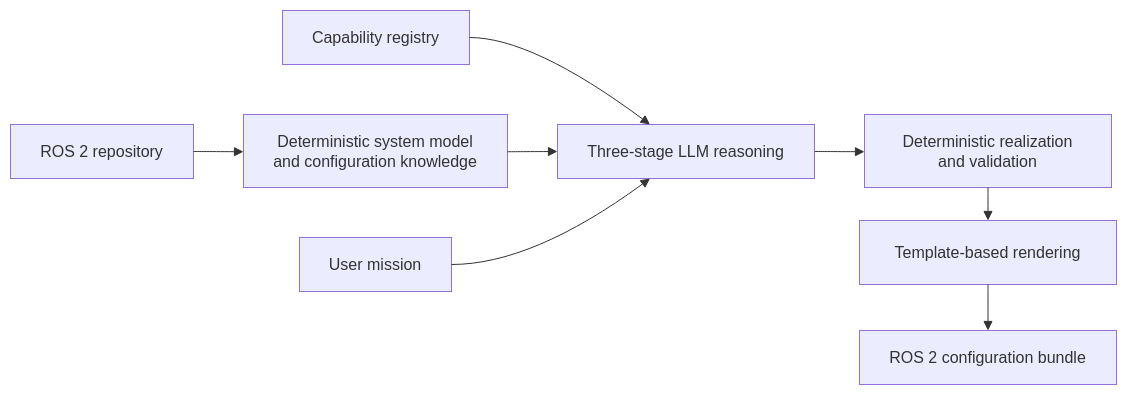
\includegraphics[width=0.96\textwidth]{pics/diagram1.png}
    \caption{Complete architecture of the proposed hybrid ROS~2 configuration framework.}
    \label{fig:proposed-complete-architecture}
\end{figure}

The proposed solution deliberately does not allow the language model to write arbitrary launch or parameter files. The model operates through structured contracts whose outputs refer to identifiers already present in the frozen configuration representation. Launch and YAML artifacts are produced only after the proposed identifiers and values have passed deterministic checks. In this way, language-model reasoning is used where semantic interpretation is required, while conventional software remains responsible for existence, type, provenance, consistency, and rendering correctness.

The first methodological requirement is to construct trustworthy knowledge about the ROS~2 project. A natural-language request cannot be mapped reliably to configuration changes if the reasoning process does not know which nodes exist, which parameters they consume, how they communicate, or which deployment path is active. The extraction stage treats the repository as a source of evidence rather than as a collection of isolated files.
Python source analysis identifies ROS-specific entities declared by the application. The extracted information includes nodes, declared parameters, parameter reads, publishers, subscriptions, services, clients, actions, timers, quality-of-service descriptions, and transform-related operations. Source locations and unresolved expressions are retained rather than discarded. This is important because later reasoning must distinguish a directly observed fact from an expression that could not be resolved statically.
Each category contributes different grounding information. A declared parameter identifies a possible control point. A parameter read and its surrounding usage provide evidence about behavioral effect. Publishers and subscriptions show how a component participates in the system and the dependency relationship with other components. Message types constrain whether two endpoints can communicate. Quality-of-service information allows the method to detect known incompatibilities.
The purpose of source analysis is not to reconstruct arbitrary Python execution perfectly. Its role is to recover a bounded set of objective ROS facts sufficient to ground configuration reasoning. When a value depends on dynamic computation or an unsupported Python pattern, the method records the unresolved expression instead of fabricating a result.
Source-level node declarations do not by themselves describe the deployed robot. ROS~2 launch descriptions determine which executables are instantiated, which namespaces and node names become effective, which conditions enable or disable them, and how launch arguments flow through included launch files. The method therefore extracts launch declarations, include relationships, launch arguments, substitutions, parameter sources, remappings, namespaces, conditions, package names and executable names.
Launch arguments are retained as configuration elements because they often control whether a subsystem is active or which implementation is selected. Conditions are preserved because the presence of a node in source code does not imply that it is enabled in the current baseline. Remappings and namespaces are resolved because communication compatibility depends on effective ROS names, not merely on the literals appearing in individual source files.
ROS parameter files provide another layer of configuration. The method extracts node selectors, nested parameter paths, scalar and structured values, and the provenance of each assignment. Wildcard selectors require special treatment. A wildcard assignment may configure several deployed nodes, but it still corresponds to one writable location in the source configuration file. The method records every affected component while preserving the fact that the value is controlled by one physical slot.
Parameter-file extraction also captures the relationship between declared defaults and deployment-time values. A parameter may have a default in Python, an assignment in YAML, and an additional launch-level source. Retaining these layers makes it possible to determine both the effective value and the location that must be modified. The output of extraction is a structured collection of observed facts, resolved values, provenance links, and explicit unresolved information.

The extracted sources describe overlapping views of the same robot. Python analysis describes possible node behavior, launch analysis describes deployment, parameter files describe configuration assignments, and package metadata describes software boundaries. The integration stage combines these views into one coherent representation of the deployed system.
The central unit of the integrated model is the deployment instance. A deployment instance connects a launch-level node action to its source-level node representation when the source is available. It records the effective node name, namespace, package, executable, activation condition, source reference, parameter sources, interfaces, and resolution status.
The distinction between a source component and a deployment instance is important. One source component may be instantiated more than once, under different names or namespaces, or may remain disabled under the selected root launch. On the other hand, a launch description may instantiate an external component for which no local source model exists. The integrated representation retains both cases.
Configuration values can originate from several layers. The method retains the declared default, YAML assignment, launch-provided parameter source, root override, and final effective value whenever those layers are available. Rather than storing only the final number or string, the model stores the ordered provenance that produced it.
Provenance has two roles. First, it supports traceability: a proposed change can be connected to the source or configuration location that controls it. Second, it supports correct application: modifying a Python default that is located inside the node definition is not equivalent to modifying a YAML assignment that overrides that default in the deployed system. The method must target the controlling physical location rather than the earliest declaration encountered during extraction.
Publishers, subscriptions, services, and other ROS entities are projected into the deployment context. Namespaces and remappings are applied to obtain effective interface names. Where sufficient local evidence exists, compatible publisher--subscription pairs are represented as confirmed communication edges. The model retains endpoint role, effective name, interface type, owning component, and available quality-of-service information.
Only relationships supported by evidence are asserted. When an endpoint belongs to an external package whose source cannot be inspected, the method records partial knowledge rather than assuming a complete connection. This conservative treatment is essential because the unified model later serves as evidence for both deterministic validation and language-model reasoning.
Every deployment instance and relationship carries an explicit resolution status. Locally resolved instances have source evidence and known extracted interfaces. External instances are represented as deployed components with unknown internal behavior. Partial or unresolved launch expressions are collected in a dedicated set of unresolved facts.
Uncertainty is therefore represented in the data. Later stages can distinguish a confirmed missing connection from one that cannot be verified because an external component has an unknown implemententation. This prevents the system from reporting certainty where the repository does not provide it.
The integrated model describes effective parameter occurrences, but configuration application requires writable physical locations. These two concepts are not always one-to-one. The method therefore projects the system model into a configuration representation whose records correspond to physical launch arguments and ROS parameter slots.
Each configuration record retains a stable identifier, source name, kind, value type, default value, current effective value, allowed values or known numerical bounds when available, provenance, modification targets, affected components, and relationships to other records. Every discovered physical slot is included as a potential configuration candidate. The method does not use a manually maintained permission policy that classifies parameters as configurable or fixed.
This design allows hardware dimensions, algorithm settings, topic names, frame identifiers, timing parameters, and launch arguments to participate in the same reasoning process. Their semantic categories may differ, but category membership does not determine whether the user is allowed to request a change. Relevance is determined for each mission, while objective validity is checked later.
When one wildcard YAML value affects multiple components, the representation contains one configuration record with multiple affected components. This prevents the reasoning process from proposing contradictory values for aliases that ultimately write to the same location.
The integrated model and the physical configuration representation are saved as frozen artifacts. Here, frozen means that they are treated as immutable inputs for a run or experiment. It does not refer to a ROS runtime feature. When source code, launch structure, parameter files, or extraction logic changes, the dependent artifacts must be regenerated in order.
This frozen boundary makes the language-model experiment reproducible. The same identifiers, values, relationships, and evidence can be supplied across repeated runs and context ablations.

\begin{figure}[htbp]
    \centering
    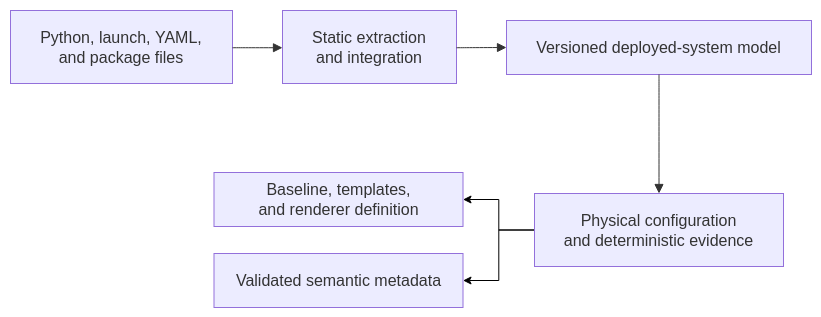
\includegraphics[width=0.90\textwidth]{pics/det_knowledge_artifact_generation.png}
    \caption{Deterministic construction of system knowledge and configuration artifacts.}
    \label{fig:deterministic-knowledge-generation}
\end{figure}

\section{Deterministic Evidence and LLM-Enriched Parameter Metadata}
Metadata is constructed for every writable physical configuration slot discovered in the analyzed deployment. The current method combines two deliberately separated sources. Deterministic repository analysis establishes parameter identity, type, current value, provenance, writable target, affected components, source evidence, and relationships directly supported by the analyzed system. A separate language-model enrichment stage derives semantic descriptions and vocabulary that are difficult to recover through syntax alone. The semantic enrichment never replaces the deterministic identity or evidence of a parameter and cannot introduce a new writable configuration slot.
The construction starts from effective parameter occurrences in the unified system model. Occurrences controlled by the same physical location are grouped into one configuration record. A ROS parameter assigned through YAML is identified by its file, node selector, and nested parameter path. A launch argument is identified by its root launch interface. This projection is necessary because one YAML wildcard may affect several deployed components, whereas configuration application must still modify that value only once.
For each resulting record, the deterministic extractor assigns a stable canonical identifier and retains the source name, configuration kind, value type, declared default, current effective value, known allowed values or numerical bounds, ordered provenance, writable target, affected components, and deterministically discovered relationships. It also creates a bounded evidence package containing source references and short excerpts for declarations, reads, and usages, together with related ROS interfaces when those interfaces can be established from the repository. Unavailable deterministic facts remain absent or explicitly unresolved; they are not inferred from the parameter name.

The semantic-enrichment model receives the bounded evidence document for one parameter per request. For each document it may produce a concise description, aliases, example user expressions, physical quantity, unit, semantic category, behavioral effects, constraints, typed relationships to other known parameters, and a confidence value. Processing one parameter at a time keeps the prompt within the configured 8192-token context and prevents the response for one parameter from being confused with another. Every response is schema-validated and saved immediately to an incremental checkpoint, so an interrupted run resumes from the last completed parameter. The frozen enrichment used in the present experiments contains one validated record for each of the 109 configuration entries. At the request of the experimental design, evidence identifiers are not required from the enrichment model and are stored as empty lists; the semantic fields must therefore be treated as uncited model-generated hypotheses rather than as source quotations. Schema validation still prevents invented parameter identities and invalid relationship targets. The enrichment artifact is hash-bound to the system model and configuration schema, so stale metadata is rejected at application start-up. Once a validated enrichment artifact is frozen for an experiment, retrieval over the combined records is reproducible even though the offline process that originally generated the semantic hypotheses used a language model.

Table~\ref{tab:deterministic-parameter-metadata} illustrates the combined record for one parameter and identifies the origin of each group of fields. The deterministic part shows why both provenance and a writable target are required: the node declares a default of \(10.0\), but the deployed YAML assignment overrides it with \(20.0\). Consequently, \(20.0\) is the current effective value and the YAML slot is the location that configuration generation must modify. The language-model part adds searchable ways of expressing the same parameter semantically, while remaining subordinate to the source-derived identity, value, target, and evidence.

\begin{table}[htbp]
\centering
\caption{Example of combined deterministic and language-model-generated metadata for a ROS parameter.}
\label{tab:deterministic-parameter-metadata}
\begin{tabular}{p{0.27\textwidth} p{0.66\textwidth}}
\hline
\textbf{Metadata field} & \textbf{Extracted value} \\
\hline
\multicolumn{2}{l}{\textit{Deterministically extracted facts and evidence}} \\
Canonical identifier & \texttt{nodes.joint\_state\_estimator.publish\_frequency} \\
Source parameter name & \texttt{publish\_frequency} \\
Configuration kind & ROS parameter \\
Value type & Floating-point number \\
Declared default & \(10.0\), extracted from the Python parameter declaration \\
Current effective value & \(20.0\), obtained after applying the YAML assignment \\
Ordered provenance & Python declaration \(10.0\) $\rightarrow$ YAML assignment \(20.0\) \\
Writable target & \texttt{src/antrobot\_ros/config/antrobot\_params.yaml}; selector \texttt{joint\_state\_estimator}; path \texttt{publish\_frequency} \\
Affected component & \texttt{joint\_state\_estimator} \\
Usage evidence & The parameter is read by the component and used to derive its periodic update interval \\
Source evidence & Stable references to the declaration, read, usage, and YAML assignment locations \\
Known constraints & Numerical type; no additional bound is recorded unless one is present in the analyzed sources \\
\hline
\multicolumn{2}{l}{\textit{Language-model-generated semantic metadata}} \\
Semantic description & The frequency at which joint-state information is published \\
Aliases & ``publish rate''; ``update frequency'' \\
Example user expressions & ``joint state update rate''; ``how often joint states are published'' \\
Physical quantity & Frequency \\
Unit & Hz \\
Semantic category & System configuration \\
Behavioral effects & Joint-state updates; odometry calculations \\
Semantic constraints & None inferred for this record \\
Typed semantic relationships & None inferred for this record \\
Semantic confidence & \(1.0\), reported by the enrichment model \\
Semantic grounding & No evidence identifiers cited in this enrichment record; the semantic fields therefore remain uncited model hypotheses \\
\hline
\end{tabular}
\end{table}

The language-model enrichment stage operates on the bounded deterministic evidence associated with one parameter. Its output is validated against a strict schema and the known parameter catalogue. In particular, relationship targets must refer to existing parameter identifiers, confidence values must lie between zero and one, and evidence references used during enrichment must originate from the supplied evidence package. Table~\ref{tab:llm-parameter-metadata} summarizes the semantic fields produced by this stage.

\begin{table}[htbp]
\centering
\caption{Semantic parameter metadata extracted by the language-model enrichment stage.}
\label{tab:llm-parameter-metadata}
\begin{tabular}{p{0.25\textwidth} p{0.68\textwidth}}
\hline
\textbf{Metadata field} & \textbf{Meaning} \\
\hline
Description & Concise natural-language explanation of what the parameter controls in the analyzed component. \\
Aliases & Alternative technical names and short expressions that may refer to the same parameter. \\
User expressions & Representative phrases an operator may use when requesting a change without naming the canonical parameter identifier. \\
Physical quantity & The measured or configured physical concept, such as distance, frequency, velocity, angle, or covariance, when applicable. \\
Unit & The semantic unit associated with the value, such as metres, hertz, seconds, or radians, when supported by the evidence. \\
Semantic category & A higher-level grouping such as robot geometry, sensor configuration, timing, navigation, or uncertainty. \\
Behavioral effect & One or more descriptions of how changing the value can affect observable system behavior. \\
Constraints & Semantic restrictions or conditions inferred from the supplied evidence, without replacing deterministically known types, allowed values, or numerical bounds. \\
Relationships & Typed links to another known parameter. Each link contains the target parameter identifier, relationship type, whether a joint update is required, a concise reason, and a confidence value. \\
Confidence & A value between zero and one representing confidence in the semantic enrichment record. \\
\hline
\end{tabular}
\end{table}

The two metadata tables are representative of the record structure, not manually authored annotations. The same deterministic extraction and semantic enrichment procedure is applied to all discovered ROS parameter slots and root launch arguments. Hardware dimensions, algorithm settings, topic and frame names, timing values, and activation arguments are therefore represented uniformly while retaining their different physical targets and source evidence. These records form the complete parameter catalogue used by the later reasoning pipeline. In the LLM-semantic retrieval variant, aliases, user expressions, descriptions, physical quantities, units, semantic categories, behavioral effects, constraints, and typed relationships provide the searchable semantic surface. Canonical identifiers, current values, types, writable targets, and provenance remain deterministic facts used for validation and application.

\section{Natural-Language Configuration Reasoning}
\label{sec:nl-reasoning}
Natural-language configuration reasoning uses at most three sequential language-model calls, with deterministic processing and validation between them. The calls have separate responsibilities:
\begin{enumerate}
    \item \textbf{Capability interpretation} determines which supported high-level robot capabilities and implementations are requested.
    \item \textbf{Parameter selection} chooses which configuration parameter identifiers are relevant from a deterministically retrieved candidate set. It does not propose new values.
    \item \textbf{Parameter value reasoning} proposes a new value for each parameter accepted after selection. It cannot introduce additional parameters.
\end{enumerate}
All three calls may use the same underlying language model, but they use different instruction prompts and structured response contracts. They are therefore separate inference calls rather than three necessarily different models. The third call is made only after a valid parameter selection, and the pipeline may terminate earlier when a preceding call reports an unsupported request, a need for clarification, or no requested parameter change. Separating the calls makes capability interpretation, parameter identification, and value derivation independently constrained and independently measurable.

% DIAGRAM PLACEMENT: insert the figure exported from
\begin{figure}[htbp]
    \centering
    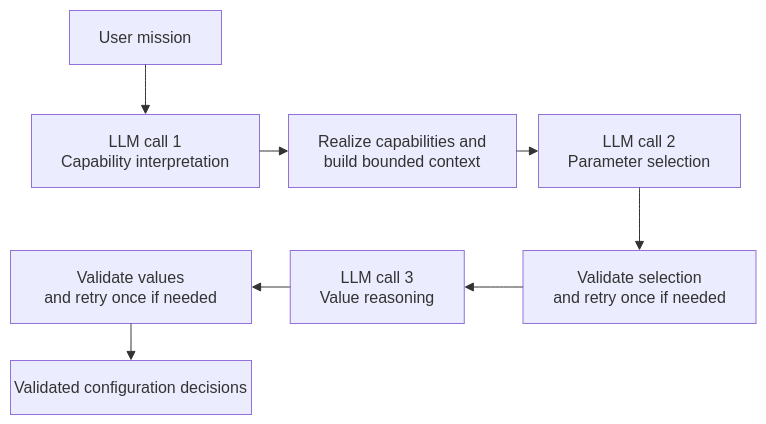
\includegraphics[width=0.72\textwidth]{pics/three_call_llm_pipeline.png}
    \caption{Three-stage language-model reasoning pipeline with deterministic processing between calls.}
    \label{fig:three-call-llm-pipeline}
\end{figure}

The capability interpreter receives the user's mission and a language-model-safe projection of the capability registry. The registry represents human-authored robot design knowledge: supported capabilities, available implementations, descriptive characteristics, and dependency information. It does not expose concrete renderer assignments to the language model. The model therefore decides what capability the user requested, not how launch files should be manipulated.
The interpretation is sparse. For each supported capability, the model may mark it as enabled, explicitly disabled, or unmentioned. When enabled, it may select a supported implementation if the request justifies a specific choice. Unmentioned and disabled are deliberately different states. An unmentioned capability preserves the baseline and creates no override. An explicitly disabled capability produces a deterministic request to disable the components belonging to that capability.
The interpreter can also return terminal outcomes. An unsupported outcome indicates that the request cannot be expressed using the available robot capabilities. A clarification outcome indicates that information required for a material decision is missing. Terminal outcomes stop the pipeline before configuration generation.
After schema validation, capability choices are expanded using the full registry. Dependency requirements are applied, conflicting capability or implementation choices are rejected, and component claims are merged deterministically. The result records active components, selected implementations, displaced implementations, required connections, concrete launch-level realization values, and provenance explaining why every claim exists.
The capability registry is validated against the frozen system before mission processing. Its component identifiers must refer to known deployed components, its realization keys must exist in the physical configuration representation, its connection endpoints must be known, and its wiring references must exist. Dependency cycles, unknown implementations, duplicate claims, and inconsistent component families are rejected before a mission is interpreted.
The realization method is intentionally bounded to the supported robot rather than formulated as a universal component-selection solver. It applies explicit capability dependencies and conflicts declared by the robot designer in order to preserve deterministic behavior. 
Required connections declared by the selected implementations are resolved against the unified system model. The method checks source and target components, publisher and subscription roles, effective names, interface types, wiring bindings, and known quality-of-service policies.
A locally known missing endpoint, incompatible interface type, unresolved required binding, or known quality-of-service incompatibility invalidates the realization. A connection involving an opaque external component may be classified as partially verified rather than falsely confirmed. The output is a mission-specific orchestration plan describing active deployment components and the verification state of required connections.
Capability realization does not filter the parameter space to active components. The complete physical configuration representation remains available because a mission may intentionally configure an implementation while enabling it, may change hardware values shared by several components, or may refer explicitly to an inactive component. Each catalogue record combines deterministic configuration facts with grounded source and system evidence.
All catalogue records remain candidates in principle, but they are not all inserted into one language-model prompt. A deterministic retrieval stage first constructs a bounded candidate set.
The mission text and searchable parameter fields are normalized and tokenized before scoring. Each parameter becomes a searchable document whose fields depend on the selected context variant.
Candidate ranking uses weighted lexical matching with inverse document frequency. Let $q$ denote the set of query tokens, $f$ a searchable field, and $p$ a parameter record. The lexical score can be summarized as

\begin{equation}
S(p,q)=\sum_{t \in q}\sum_f
w_f \cdot \operatorname{idf}(t) \cdot
\left(1+\log c_{p,f}(t)\right),
\end{equation}

where $c_{p,f}(t)$ is the number of occurrences of token $t$ in field $f$, and $w_f$ gives greater importance to discriminative fields than to generic text. In the semantic configuration, aliases have weight 2.5 and example user expressions have weight 2.0; an exact alias phrase, parameter identifier, or source name receives an additional exact-match bonus. The ranking is deterministic: the same frozen mission-specific catalogue, request, and retrieval configuration produce the same candidate order.
The highest-ranked candidates are retained up to a configured limit. Under the \texttt{graph} and \texttt{metadata\_graph} variants, the method then follows eligible explicit parameter relationships and shared wiring bindings for a bounded number of hops. Graph neighbors receive a discounted score and retain the identifier of the candidate through which they were discovered. This allows a lexical match for one occurrence of a shared concept, such as wheel radius, to introduce another physically related occurrence when both consuming components are active, even when the second record shares fewer words with the request.
Lexical retrieval is intentionally a transparent baseline rather than a claim of full semantic search. It searches semantically meaningful fields, but the matching operation itself remains token based. The language model performs semantic selection only after this deterministic candidate construction.
Retrieved records are serialized in rank order under a fixed character budget. The context records which identifiers were included, which candidates were omitted because of the budget, how each record was retrieved, and which relationship edges are relevant.
This bounded construction provides a reproducible context window and a measurable retrieval boundary. If a correct parameter is absent from the supplied context, the failure can be attributed to retrieval rather than to parameter selection.
The parameter-selection model receives the original mission, the complete compact metadata for each bounded candidate, a concise summary of the decided capabilities and active components, relevant wiring bindings, and a strict structured-output contract. This call uses a 16384-token context window, while capability interpretation and value reasoning retain the 8192-token setting. It must either select one or more supplied parameter identifiers or return a terminal status indicating no parameter change, unsupported intent, or a need for clarification.
For a valid selection, the model returns each selected parameter identifier together with a concise relevance explanation and, when available, identifiers for the grounding evidence it used. Deterministic validation rejects identifiers absent from the supplied context, duplicate identifiers, and evidence references that were not provided for that parameter. The language model therefore cannot introduce a parameter directly from the full catalogue or fabricate a source citation.
Value reasoning is invoked only after a valid selection. It receives the original mission, the validated selection, the selected parameter records, their current values, their known constraints, and relevant relationships. It does not receive the full catalogue. Its task is to propose a new value for each required parameter and give a concise, externally verifiable reason.
Separating selection from value reasoning prevents the model from hiding an incorrect parameter choice inside an otherwise plausible numerical answer. It also permits independent evaluation of whether the system found the right configuration elements and whether it derived the right values.
The value stage may return a clarification or unsupported result if the selected context does not contain enough information to determine a responsible change. For a valid result, every proposed change must repeat the current value observed in the frozen catalogue. This old-value check prevents a response generated against stale context from being applied silently.

\begin{figure}[htbp]
    \centering
    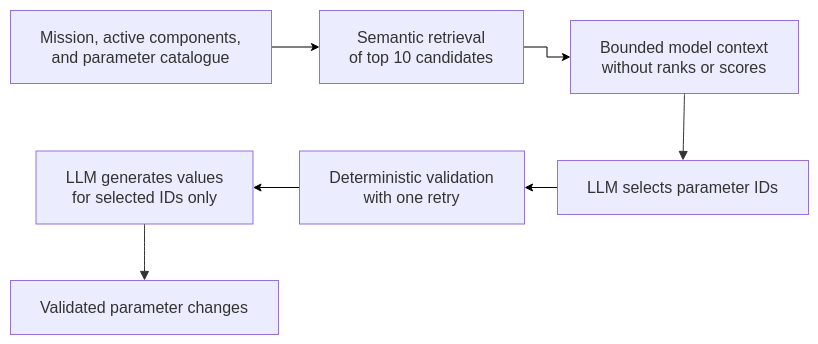
\includegraphics[width=0.90\textwidth]{pics/4parameter_retrieval.png}
    \caption{Bounded parameter retrieval followed by separated selection and value reasoning.}
    \label{fig:parameter-retrieval-reasoning}
\end{figure}

\section{Configuration Plan Generation and Validation}
\label{sec:plan-validation}
The conclusions of the language-model stages are not applied directly to files. They are converted into explicit intermediate plans that form a deterministic boundary between inference and system modification.
The first intermediate representation is the system realization produced from capability choices. It contains component activation claims, selected implementations, dependencies, required ROS connections, launch-level realization values, and provenance. The second representation is the validated set of parameter changes produced after selection and value reasoning. These two sources are merged into one sparse configuration plan.
The plan is sparse by design. It contains only values that differ because of the current mission. Unmentioned capabilities, unchanged parameters, and unrelated baseline values are not copied into it. Sparsity makes the causal effect of the request visible and reduces the risk that a model-generated response accidentally rewrites the complete configuration.
Every planned value is addressed by a canonical identifier from the physical configuration representation. Capability realization and parameter reasoning may target the same identifier only when they agree on the value. If, for example, capability realization requires an implementation to be enabled while parameter reasoning proposes disabling its launch argument, the plan is rejected instead of resolving the conflict through update order.
The plan also retains evidence and provenance. Capability values record which selected or required capability produced them. Parameter values retain the user's request and the model's concise justification. This information supports audit, failure analysis, and user-facing explanation without requiring access to hidden model reasoning.
Introducing this representation has several methodological advantages. It prevents direct language-model file editing, establishes a stable contract for validation, allows the same plan to be rendered through different output strategies, and makes the proposed change independently inspectable before application.
Validation is distributed across the method so that each stage checks the properties for which it has sufficient information. The validator does not attempt to replace semantic reasoning with an extensive hand-written configuration policy. Instead, it verifies objective properties that can be established deterministically.
At application start-up, the system model, physical configuration representation, renderer manifest, and parameter evidence are checked for supported schema versions. The evidence artifact contains hashes of the system and configuration models from which it was derived. A mismatch marks the artifact as stale and prevents its use.
The capability registry is cross-validated against these artifacts. Component identifiers, implementation references, realization keys, required connection endpoints, and wiring bindings must resolve. Dependency cycles and inconsistent declarations are rejected before mission processing.
Every language-model output must conform to its structured response contract: capability selections may contain only supported capability and implementation values, sparse-state invariants prevent an implementation from being named unless its capability is enabled, parameter selection is constrained to identifiers and evidence supplied in the bounded context, and value reasoning cannot introduce a parameter that was not selected or propose a value inconsistent with the parameter's declared type, allowed values, or known bounds. These checks establish that the model's result is grounded in the current retrieval output and the frozen catalogue; they do not assert that its semantic choice is correct. Section~\ref{sec:config-gen-validation} details how each of these checks is implemented.
Where multiple effective parameter occurrences are controlled by one physical slot, the slot representation prevents divergent proposals by construction. Where separate physical slots are related, the relationship is supplied as reasoning context and can be evaluated as part of the task annotation; the system does not impose a universal rule that every semantically related parameter must always have the same value.
The merged plan is checked against the complete physical configuration representation and the renderer interface. Every key must exist and be renderable. Capability and parameter claims targeting the same key must agree. The plan remains sparse, but the resolved rendering context must become complete after it is overlaid on the baseline. Generated artifacts then pass structural checks and, optionally, a more expensive offline equivalence analysis, detailed alongside the renderer implementation in Section~\ref{sec:config-gen-validation}.
These validation layers establish structural and factual correctness. They do not claim to prove that every semantically plausible parameter change is physically safe for every robot or environment. Such domain assurance requires additional system-specific constraints or experimental validation.

\begin{figure}[htbp]
    \centering
    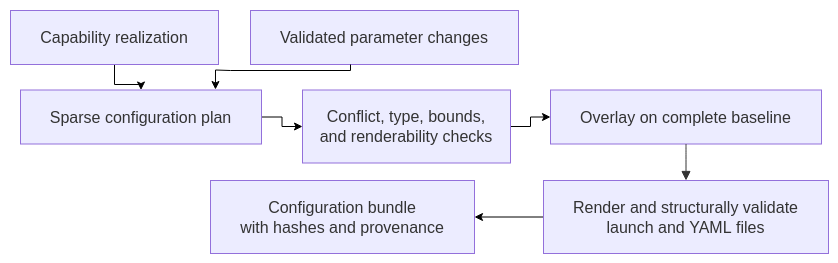
\includegraphics[width=0.90\textwidth]{pics/sparse_plan_validation.png}
    \caption{Validation and deterministic application of the sparse configuration plan.}
    \label{fig:sparse-plan-validation}
\end{figure}

\section{Configuration Application and End-to-End Workflow}
Once the sparse plan has passed the validation described in Section~\ref{sec:plan-validation}, it is overlaid on the complete baseline and materialized through the predefined launch and parameter templates introduced above; the language model never produces launch syntax, YAML structure, output paths, or installation targets. Application produces a mission-specific launch wrapper, parameter files, a record of resolved values and merge provenance, a manifest of generated files, and structural validation results. The method stops at artifact production: it does not start ROS~2 nodes, install packages, or claim that generated behavior has been validated on a physical robot, and Section~\ref{sec:config-gen-validation} details the renderer implementation.

Consider the request: ``Build a map using KISS-ICP and limit its range to 20 metres.'' This request combines a high-level capability choice, an implementation choice, and a lower-level algorithm parameter change, making it representative of the complete method and showing how the stages defined in the preceding sections act together.

Before the request is processed, the repository has already been analyzed: the frozen system model identifies the deployed mapping, laser, odometry, and conversion components, and the capability registry declares mapping and odometry as supported capabilities with KISS-ICP as one available odometry implementation.

The capability interpreter maps ``build a map'' to the mapping capability and ``using KISS-ICP'' to the KISS-ICP odometry implementation; it does not attempt to turn ``20 metres'' into a capability, leaving that phrase for the parameter-reasoning stages. Deterministic realization then activates mapping, activates KISS-ICP together with the laser-scan-to-point-cloud conversion it requires, displaces the alternative kinematic ICP implementation, and checks the resulting sensor-to-odometry chain against the frozen system model; a confirmed structural incompatibility would stop the request before parameter reasoning.

Bounded retrieval ranks the complete catalogue using the mission terms, so records associated with the KISS-ICP range are expected to rank highly. The selection model receives only this retrieved context and selects the maximum-range parameter -- and only that parameter, not unrelated mapping frequencies, frame names, or topic parameters -- because the request explicitly limits the implementation's sensing range. The value model then receives the selected record, its current value, type, and constraints, and proposes a new value of 20 metres, explained as directly stated by the user; the reported old value and the new value are checked against the frozen catalogue as described in Section~\ref{sec:plan-validation}.

The validated parameter change is merged with the launch-level values from capability realization into a sparse plan containing only the values needed to activate mapping, select KISS-ICP and its dependency, displace the alternative implementation, and set the requested maximum range. After the checks described above, the plan is overlaid on the complete baseline and rendered; the resulting files are checked structurally and packaged with traceability information. At no point does the language model directly edit a ROS file or select an output path.

This example illustrates the intended division of responsibility: the language model maps natural language to supported capabilities, relevant parameters, and requested values; deterministic representations establish what exists; deterministic realization expands robot-specific design knowledge; and deterministic validation and rendering ensure that the conclusion can be applied to the modeled system.

\begin{figure}[htbp]
    \centering
    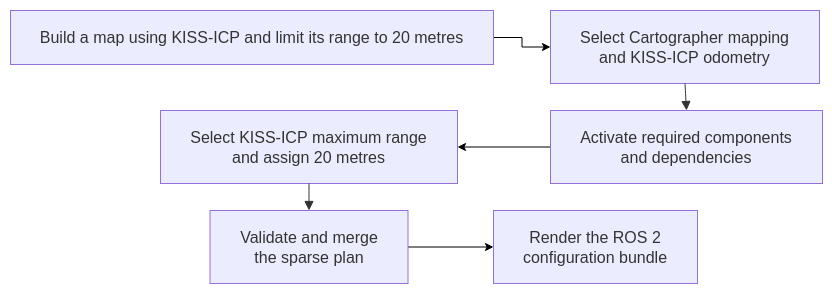
\includegraphics[width=0.90\textwidth]{pics/end_to_end_request.png}
    \caption{Processing of a representative mapping and KISS--ICP configuration request.}
    \label{fig:representative-end-to-end-request}
\end{figure}

\section{Limitations and Design Boundaries}
The proposed method intentionally adopts several boundaries in order to keep the research focus on source-grounded language-model reasoning.
First, static analysis is incomplete by nature. Dynamically generated node names, reflective Python behavior, runtime-created interfaces, environment-dependent substitutions, and unsupported language patterns may remain unresolved. The method exposes these limitations explicitly but cannot infer facts absent from the analyzed repository.
Second, external ROS packages may appear in launch descriptions without locally available source code. Their deployment presence can be represented, but their internal parameters and interfaces cannot be validated to the same degree as local components. Connections involving such packages may remain partially verified until runtime information or additional package models are provided.
Third, the capability registry is human-authored robot design knowledge. The method validates its references and internal consistency, but it does not discover autonomously which high-level capabilities a robot should support or which implementation combinations are desirable. The registry is deliberately small and robot-specific rather than a universal ontology of ROS functionality.
Fourth, the retriever remains lexical even when language-model-generated metadata is enabled. It searches deterministically extracted fields together with frozen descriptions, aliases, example user expressions, and semantic relationships, but candidate matching still depends on normalized token and phrase overlap. Incorrect or incomplete enrichment can therefore mis-rank a candidate, while a concept absent from every searchable field may still be missed. Embedding, hybrid, or learned retrieval can be evaluated later as separate methods, but they are not silently assumed by the proposed method.
Fifth, structural validation cannot guarantee physical safety or behavioral success. Type correctness, known bounds, valid ROS names, and compatible interfaces are objective checks; deciding whether a change is appropriate for a particular robot, environment, or safety envelope may require additional domain constraints, simulation, or hardware experiments.
Sixth, the method produces deployable configuration artifacts but does not itself launch, monitor, or recover the ROS~2 system. Runtime lifecycle management, distributed deployment, fault recovery, and automatic rollback are outside the proposed configuration-reasoning boundary.
Finally, structured generation cannot eliminate semantic errors; bounded context, validation, abstention, and deterministic application limit their consequences.

\chapter{Implementation Details}
\section{Implementation Overview}
The prototype was implemented primarily in Python and operates directly on a ROS~2 workspace. Its organization follows the hybrid architecture introduced in the previous chapter: deterministic modules extract and integrate repository facts, a language-model layer performs bounded semantic reasoning, and deterministic validation and rendering modules convert accepted decisions into ROS~2 configuration artifacts. The implementation avoids executing the analyzed source code, allowing repository analysis to remain independent of an installed or running ROS graph.
Python's Abstract Syntax Tree infrastructure is used to analyze ROS node and launch source files. Structured intermediate representations are validated with Pydantic and serialized as JSON artifacts. ROS parameter files are read as YAML mappings, with a dependency-free parser for the supported ROS subset when an external YAML package is unavailable. Jinja2 with strict undefined-variable handling is used to materialize launch and parameter files. Local language-model inference is accessed through Ollama's chat endpoint using structured JSON schemas and deterministic temperature settings.
The application is controlled through one flat configuration document located beside the orchestration module. It selects one of three operations: repository analysis, validation of an existing system model, or processing of a natural-language mission. The same document defines artifact paths, prompt paths, the Ollama model, retrieval limits, and output locations. Unknown or invalid fields are rejected before the selected operation begins.
The repository implementation is divided according to responsibility rather than according to individual experiments. Extraction modules produce source, launch, and configuration facts. Integration modules create the deployed-system representation. Mission modules implement capability interpretation, retrieval, parameter selection, value reasoning, and evaluation contracts. Templating modules derive the physical configuration interface and render output artifacts. Validation modules check the system model and generated scenarios. This structure preserves a one-way dependency flow from schemas and extraction toward integration, reasoning, rendering, and validation.

\section{ROS 2 Information Extraction}
ROS node extraction is implemented as static AST analysis. Every Python source file under the selected workspace roots is parsed without importing or executing it. Files in build, installation, log, virtual-environment, cache, and version-control directories are ignored. Parse failures are retained in the output rather than terminating analysis of the remaining repository.
The extractor first preserves ordinary Python facts, including imports, module assignments, classes, methods, functions, entry points, conditions, and loop contexts. A second interpretation step identifies ROS-specific constructs. It recognizes node classes and common factory calls for parameters, publishers, subscriptions, services, clients, timers, action clients and servers, quality-of-service profiles, and transform utilities. For example, a declaration such as

\begin{verbatim}
self.declare_parameter("wheel_radius", 0.03)
\end{verbatim}

is represented as a parameter named \texttt{wheel\_radius}, with a numerical default and a source location. Calls that read the same parameter are associated with the declaration, allowing later evidence construction to include both where the parameter is exposed and how its value is used.
A small static resolver evaluates expressions that are safe and repository-local. It supports literals, names with known assignments, lists, tuples, dictionaries, unary operations, selected binary operations, and formatted strings whose components can be resolved. Import aliases are qualified so that ROS calls can be recognized even when modules or symbols are renamed locally. Assignments are processed iteratively because the value of one expression may depend on an earlier symbol.
When an expression cannot be evaluated, the extractor stores its textual form, symbolic dependencies, and resolution status. Conditional and loop contexts are also preserved. This approach is intentionally conservative: a dynamic expression remains explicit evidence of incomplete resolution rather than being replaced with a guessed value. Stable identifiers derived from source location and entity kind make extracted records reproducible across repeated runs on unchanged source.
ROS~2 launch files are Python programs, so they are analyzed through a dedicated AST resolver rather than executed. The extractor recognizes launch arguments, node actions, included launch descriptions, launch configurations, package-share substitutions, path substitutions, node parameter sources, remappings, command-line arguments, namespaces, and conditional actions.
Assignments are resolved iteratively before launch actions are interpreted. The launch resolver retains structured representations for substitutions that cannot be reduced immediately. For example, a launch argument reference remains identifiable as a launch-configuration dependency even when its final value is supplied by a parent launch file.
Each launch file initially produces a local record. During system integration, include relationships are followed recursively from the configured root launch file. Arguments supplied by a parent include are propagated into the child context, and root overrides take precedence over inherited or declared defaults. The implementation therefore distinguishes files that merely exist in the repository from actions that participate in the selected deployment.
For each deployed node action, the extractor retains package, executable, requested name and namespace, parameter sources, remappings, launch arguments, condition, and source location. This information is later matched with source-level node facts. Unresolved launch expressions and missing include targets are reported explicitly.
Parameter-file extraction scans YAML files under the selected source roots and accepts top-level mappings that contain ROS \texttt{ros\_\_parameters} entries. The parser handles scalar, list, and nested mapping values. Nested parameter dictionaries are flattened into addressable parameter paths while the original hierarchy is preserved for rendering.
Each profile records its source file, node or namespace selector, parameter mapping, flattened values, and a stable identifier. Ordinary node selectors and wildcard selectors are supported. A wildcard assignment is represented once as a physical YAML location and may later be associated with several deployment instances. This prevents the same source value from being exposed as several independently writable aliases.
Together, the three extractors provide complementary views. Python analysis establishes what a node declares and how values participate in its behavior. Launch analysis establishes what is deployed and which substitutions, namespaces, remappings, and conditions are effective. YAML analysis establishes which values are supplied to the deployed components. None of these views is sufficient independently; the system model is produced by resolving them together.

\section{System Model Construction}
System-model construction begins with the selected root launch file and recursively resolves its include graph. Each node action becomes a deployment instance. Local deployment instances are matched to source-level ROS node records using package, executable, entry-point, and node-name information. Components whose implementation is not available in the workspace remain external deployment instances with unknown internal interfaces.
Parameter resolution combines declaration defaults with launch and YAML configuration sources. The resulting record retains both the effective value and an ordered provenance chain. Consequently, the implementation can distinguish a Python declaration from the YAML assignment that controls the deployed value. This provenance is later projected into parameter evidence and into the modification targets used by the renderer.
Launch conditions are evaluated under the propagated argument context to determine the baseline activation state. Effective node names and namespaces are resolved from launch declarations. Publishers and subscriptions discovered in source code are then projected into the deployment context by applying namespaces, parameter-driven topic values, and remappings. The same process retains message types, endpoint roles, owning instances, and quality-of-service descriptions where available.
Confirmed local communication edges are created only when publisher and subscriber endpoints have compatible effective names and interface types. For example, the current AntRobot model confirms the wheel-odometry connection between the drive component and the joint-state estimator. External interfaces are not inferred from package names alone, so connections involving opaque packages remain partially known.
The integrated representation also records include relationships, launch-argument flow, source inventories, unresolved facts, and validation coverage. A system-model validator checks unique deployment identifiers, interface references, connection endpoints, local source evidence, parameter uniqueness, and parameter provenance. External components are permitted to have unknown interfaces by design, while a locally resolved instance without source evidence is treated as an error.
The effective-parameter representation is subsequently projected into physical configuration slots. Launch arguments are retained when they are forwarded by the root launch interface. ROS parameters are grouped by their controlling YAML target. Each slot records its canonical key, type, current and default values, provenance, target, affected components, relationships, and any extracted bounds. The current prototype derives 109 writable physical slots from 114 effective parameter occurrences, illustrating why effective occurrences and writable locations must remain separate concepts.

\section{LLM Integration and Context Construction}
The language-model integration uses Ollama as a local inference service. Requests are sent to the chat endpoint with a system message, a user message, temperature zero, and a JSON schema corresponding to the expected response type. The model response is accepted only as a single JSON object and is then validated against the relevant Pydantic contract. Surrounding prose, invented fields, malformed JSON, and schema-incompatible values are rejected.
Three structured model calls are used during a mission. Capability interpretation produces a sparse selection over supported capabilities and implementations. Parameter selection chooses relevant parameter identifiers from a bounded candidate context. Value reasoning proposes new values only for the validated selection. Each call uses a response schema specific to its task.
The capability instruction context is assembled from a versioned prompt template and a safe projection of the human-authored capability registry. This projection exposes descriptions, implementation choices, and characteristics but hides concrete renderer values. During one application run, the resulting capability instruction context remains stable while the user mission changes.
Parameter reasoning requires request-specific context. A deterministic lexical retriever first scores every parameter in the complete catalogue against the mission. Searchable fields are selected by the configured context variant and may include identifiers, source names, components, values, source excerpts, ROS interfaces, and relationships. Exact parameter-name occurrences receive the highest priority, while other matches use field weighting and inverse document frequency. By default, the highest twelve lexical candidates are retained.
In the graph variant, the initial candidates are expanded through extracted parameter relationships and shared topic or frame bindings. Expansion is limited by a configured hop count and a maximum of twenty-four candidates. The ranked records are then serialized under a 40,000-character budget. Each record includes its retrieval score, origin, and available evidence identifiers, making the candidate boundary reproducible and inspectable.
The final selection context combines the candidate records with the current capability realization and ROS orchestration status. Its instruction template is stable, but the inserted context changes for every mission. The selection response may represent a valid set of parameter identifiers, no requested parameter change, an unsupported request, or a need for clarification. Selected identifiers must occur in the supplied context, and cited evidence must belong to the corresponding records.
Value reasoning receives only the selected records, their current values, known constraints, and relevant relationships. This second prompt is also assembled per request. Separating the two calls allows selection quality and numerical reasoning quality to be evaluated independently and prevents the value stage from introducing a parameter that was never selected.

\section{Configuration Generation and Validation}
The nondeterministic boundary ends at structured capability and parameter conclusions. Capability choices are expanded deterministically through the validated capability registry. This expansion resolves required capabilities, selected and displaced implementations, component claims, required ROS connections, and concrete launch-level values. Required connections are checked against effective endpoints, interface types, topic or frame bindings, and known quality-of-service policies before parameter changes are considered executable.
The parameter-selection response is validated against the bounded context. The value response is then checked against the selection and complete catalogue. Every proposal must identify a selected parameter, repeat the frozen current value, and supply a new value compatible with the parameter type, allowed set, and known numerical bounds. Duplicate or unknown identifiers are rejected.
Validated capability values and parameter changes are merged into a sparse configuration plan. The plan contains only values affected by the current mission. If both sources target the same canonical key, their values must agree. This prevents update order from hiding a contradiction, such as capability realization enabling an implementation while parameter reasoning attempts to disable the same launch argument.
The renderer begins with a generated baseline containing every physical configuration key. Optional scenario values and the mission plan are overlaid in a fixed order, and each stage is recorded as provenance. Before rendering, profile and mission values are validated against the configuration schema; after merging, the resolved context must contain every required key.
Jinja2 templates are evaluated using strict undefined-variable behavior. The generated template definition has exact set equality between schema keys, baseline keys, and template references. Launch values are serialized into a wrapper launch description, while ROS parameters are written into package-overlay YAML files at predetermined targets. The LLM therefore never produces Python launch syntax, YAML structure, file paths, or installation routes.
Generated launch files are parsed as Python, and generated YAML files are checked for a top-level mapping and valid ROS parameter sections. Each rendered file receives a SHA-256 digest and a record of its template, output route, deployment strategy, and referenced keys. Mission-time rendering performs these structural checks without reanalyzing the entire repository. A more expensive offline equivalence mode installs the generated overlay in an isolated analysis workspace, rebuilds the system model, and compares the active deployment and communication projections with the frozen reference.

\section{Testing and Reproducibility}
The test suite is organized into unit, integration, scenario, and equivalence levels. Unit tests cover Python and deployment extraction, configuration-slot construction, capability interpretation and realization, retrieval, parameter selection, value validation, template definition, application configuration, synthetic-data handling, and evaluation metrics. Integration tests construct the AntRobot system model and execute the mission pipeline with controlled model responses. Scenario tests verify that only declared configuration deltas are accepted. Equivalence tests confirm deterministic rendering, baseline preservation, physical-slot consistency, and optional reanalysis of generated bundles.
At the current implementation checkpoint, 59 tests execute successfully. This number is reported only as an implementation sanity check; language-model accuracy is evaluated separately through the dissertation's experimental protocol.
Deterministic artifacts are regenerated through one canonical workflow in dependency order: system model, physical configuration schema, templates and baseline, parameter evidence, and scenario bundles. The workflow removes stale generated directories rather than mixing outputs from different versions. A generation record stores schema versions, artifact counts, equivalence settings, and SHA-256 hashes for the produced files. Parameter evidence additionally stores hashes of its direct input models.
The current AntRobot artifact contains 12 deployment instances, of which four are locally resolved and eight represent external components. Seven instances are enabled in the baseline. The model contains 114 effective parameter occurrences, nine known local interfaces, one confirmed local communication edge, and one explicitly unresolved deployment fact. Its validation report contains no structural errors. The physical configuration projection contains 16 launch arguments and 93 ROS parameter slots, for a total of 109 writable values. These figures demonstrate that the complete generation pipeline executes on the target workspace; they are not presented as language-model performance results.
Reproducible LLM experiments retain the model identifier, prompt versions, context variant, retrieval limits, graph depth, dataset version, frozen artifact hashes, raw predictions, and structured errors. Temperature zero reduces sampling variability, while repeated-run reporting remains necessary because identical generation is not guaranteed across model versions, inference runtimes, or hardware environments.

\chapter{Dataset and Experimental Results}
\label{chap:dataset-results}

This chapter describes the construction of the AntRobot natural-language mission datasets, the evaluation protocol used for the language-model stages, and the progression from the initial prompt baselines to semantic parameter metadata. Configuration rendering, generated YAML files, and generated launch files remain outside the scope of these experiments; only capability interpretation, parameter retrieval, parameter selection, and parameter-value reasoning are evaluated.

\section{Dataset construction}

The dataset was constructed in the direction from a verified structured intent to natural-language expressions. This direction was chosen to keep the reference label independent of the text-generation model. The model generated linguistic variants of an existing annotation; it did not generate the expected capability or parameter answer.

The construction process consisted of the following stages:

\begin{enumerate}
    \item Fifteen seed missions were defined from capabilities and parameters that exist in the extracted AntRobot system model. Each seed contains a canonical intent, a sparse capability annotation, any explicitly requested parameter values, and category labels used for grouped evaluation.
    \item For each seed, the local \texttt{qwen2.5-coder:7b} model generated ten paraphrases. The requested styles included canonical language, natural language, shorthand+, imperative phrasing, negative phrasing, and multi-clause requests.
    \item Automatic checks rejected malformed records, duplicate texts after normalization, and records that violated the candidate schema.
    \item A semantic review checked that each paraphrase preserved the seed intent and did not add or remove requirements. Rejected variants were regenerated or replaced. The generation history and rejected texts were retained rather than overwritten.
    \item Fourteen records required a manual language repair after semantic review. The final dataset therefore contains 136 model-generated paraphrases and 14 repaired paraphrases.
    \item The final JSON Lines file was frozen together with generation metadata, raw responses, rejection logs, and repair logs.
\end{enumerate}

The reference annotations are copied from the repository-grounded seed missions. Consequently, the generator cannot improve its evaluation score by placing an answer in the generated text that was not already present in the seed. Nevertheless, the current paraphrase set is marked \texttt{assistant\_reviewed\_pending\_author\_review}. The reported results should therefore be treated as the first experimental baseline and not yet as a final independently verified benchmark result.

\subsection{Dataset contents}

The resulting \texttt{antrobot\_mission\_dataset\_v1.jsonl} file contains 150 missions: 15 intent groups with 10 paraphrases per group. Every record contains a stable identifier, a source-seed identifier, the natural-language mission, the expected capability interpretation, and the expected parameter values. All 150 missions in this version are supported requests. Unsupported and ambiguous requests are therefore not represented in this first benchmark, and safety metrics for those outcomes cannot yet be estimated.

Table~\ref{tab:dataset-composition} summarizes the main task composition. The categories are mutually exclusive at seed level.

\begin{table}[H]
\centering
\caption{Composition of the AntRobot mission dataset.}
\label{tab:dataset-composition}
\begin{tabular}{p{4.2cm}p{7.8cm}rr}
\toprule
Task family & Examples of covered behavior & Seeds & Missions \\
\midrule
Capability only & mapping, navigation, exploration, odometry selection, explicit disabling & 7 & 70 \\
Parameter only & publication frequency, wheel radius, wheel separation, encoder resolution & 4 & 40 \\
Capability and parameter & exploration rates, KISS-ICP range, mapping with parameter constraints & 4 & 40 \\
\midrule
Total & & 15 & 150 \\
\bottomrule
\end{tabular}
\end{table}

The dataset covers sparse requests, multi-capability requests, explicit negation, implementation selection between kinematic ICP and KISS-ICP, physical-unit conversion, and synchronized changes to multiple parameters that represent one physical property. For example, a wheel-radius request must update both the drive node and the joint-state estimator, while a request expressed in centimetres must be converted to metres.

A separate five-case file, \texttt{evaluation\_missions.jsonl}, is retained as a small diagnostic set. It is useful for quickly detecting regressions, but its size is insufficient for standalone statistical conclusions. The 150 generated missions form the main dataset for the baseline reported below.

\subsection{Parameter-reasoning challenge set}

A second file, \texttt{parameter\_reasoning\_tasks\_v1.jsonl}, was introduced to isolate the retrieval, selection, and value boundaries that the first experiments identified as the main bottleneck. It contains 40 cases: 28 requests with concrete parameter changes, four capability-only or preservation requests that should produce \texttt{no\_change}, four ambiguous requests that should request clarification, and four requests for parameters absent from the extracted robot model that should be rejected as unsupported. Table~\ref{tab:parameter-challenge-composition} gives the difficulty distribution.

\begin{table}[H]
\centering
\caption{Composition of the parameter-reasoning challenge set.}
\label{tab:parameter-challenge-composition}
\begin{tabular}{p{4.0cm}p{8.0cm}r}
\toprule
Difficulty & Main behavior & Cases \\
\midrule
Explicit & Direct parameter name and target value & 7 \\
Semantic & Paraphrase, relative value, or period--frequency reasoning & 7 \\
Physical & Unit conversion and coupled physical parameters & 4 \\
Behavioral & Desired effect rather than the source parameter name & 6 \\
Multi-component & Coordinated topic, frame, or covariance changes & 4 \\
No change & Capability-only, informational, or preservation request & 4 \\
Ambiguous & Missing target, component, or value & 4 \\
Unsupported & Requested setting is absent from the robot model & 4 \\
\midrule
Total & & 40 \\
\bottomrule
\end{tabular}
\end{table}

All 40 challenge records are currently marked \texttt{pending\_human\_review}. Experiments using this file are consequently reported as development results, not as final benchmark claims. The evaluation command requires an explicit override to run on these pending annotations, preventing accidental presentation of them as human-verified ground truth.

\section{Evaluated language-model pipeline}

The application uses one model in three specialized calls, rather than three independently trained models. All calls in the baseline use \texttt{qwen2.5-coder:7b} with temperature zero, but each call has a distinct system prompt and structured response schema:

\begin{enumerate}
    \item \textbf{Capability interpretation} identifies mapping, navigation, exploration, and odometry requirements and chooses an overall status.
    \item \textbf{Parameter identification} receives a bounded, retrieved parameter context and selects the identifiers that must change.
    \item \textbf{Value reasoning} receives the selected parameters and proposes their new values. This call is skipped when the second stage returns \texttt{no\_change}, \texttt{unsupported}, or \texttt{needs\_clarification}.
\end{enumerate}

In the current implementation, the first call is followed by deterministic capability realization. The realized active-component set restricts the parameter catalogue before retrieval: node parameters belonging only to inactive components and all launch arguments are excluded, while relationships to excluded parameters are pruned. The second call therefore chooses only among parameters belonging to the capability implementation already selected by the first call. The historical experiments below are labelled when they predate this restriction. Every experiment stops after the third language-model boundary; it does not construct a configuration plan, render YAML, assemble launch files, or score rendered artifacts.

For reproducibility, each prediction stores the exact system prompt, user prompt, raw response, parsed structured object, latency, failure stage, and validation error. The experiment metadata additionally freezes hashes of both datasets, the three prompt templates, capability registry, system model, parameter evidence, configuration schema, and application configuration.

\section{Evaluation metrics}

The metrics distinguish partial semantic understanding from an entirely correct structured prediction.

\subsection{Outcome accuracy}

Outcome accuracy is the proportion of missions assigned the correct terminal status. The possible capability-stage outcomes are \texttt{valid}, \texttt{unsupported}, and \texttt{needs\_clarification}. Since the 150-mission paraphrase benchmark contains only supported missions, its outcome metric measures valid-request acceptance and does not measure unsafe acceptance of unsupported requests. The separate parameter challenge set adds unsupported and ambiguous outcomes.

\subsection{Capability metrics}

Capability exact match requires the complete sparse capability object to equal the reference annotation. Any missing capability field, extra field, wrong implementation, or incorrect selection basis makes the case incorrect. Capability micro precision and recall instead compare individual field--value pairs over the full dataset. Their harmonic mean is

\begin{equation}
F_1 = 2 \cdot \frac{P \cdot R}{P + R},
\end{equation}

where $P=TP/(TP+FP)$ and $R=TP/(TP+FN)$. Micro aggregation sums true positives, false positives, and false negatives before computing the score, giving each annotated field equal weight.

\subsection{Parameter-selection metrics}

Parameter-selection exact match requires the predicted parameter-ID set to equal the expected set. Selecting a graph-adjacent but unnecessary parameter, omitting one occurrence of a shared physical parameter, or inventing an identifier all cause exact-match failure. Micro precision, recall, and $F_1$ provide partial credit per parameter identifier across the dataset.

Retrieval recall at rank $k$ is the fraction of expected parameter identifiers present among the first $k$ ranked candidates. Mean reciprocal rank (MRR) averages the inverse rank of each expected identifier, so an expected parameter at rank one contributes $1$, at rank two contributes $1/2$, and a missed parameter contributes $0$. These metrics are computed before language-model selection and therefore distinguish retrieval failure from selection failure.

\subsection{Parameter-value metrics}

Parameter-value exact match requires the complete expected identifier--value mapping. Numeric values are evaluated after the annotated unit conversion. The value result is downstream of parameter identification: if the correct identifier is not selected, the value model cannot produce a correct value for it. The present end-to-end value metric therefore measures the combined effect of selection and value reasoning. A later oracle-selection experiment should supply the gold parameter IDs to isolate value-reasoning ability.

\subsection{Joint correctness, completion, robustness, and latency}

Joint LLM exact match requires the correct outcome, an exact capability object, an exact parameter set, and exact values for all applicable stages. Validated inference completion measures whether all required calls returned outputs that passed JSON, schema, bounded-context, identifier, and value validation; completion does not imply semantic correctness.

For the parameter challenge set, outcome accuracy measures whether the pipeline returned \texttt{valid}, \texttt{no\_change}, \texttt{needs\_clarification}, or \texttt{unsupported} as annotated. End-to-end accuracy additionally requires exact parameter selection and an exact complete value set. Unsafe execution rate is the fraction of ambiguous and unsupported requests for which the pipeline nevertheless returned \texttt{valid}; lower is better, and $0\%$ is the desired result.

For the generated dataset, paraphrase consistency is the fraction of seed groups for which all ten variants produce the same structured outputs. Group robustness is stricter: all ten variants must be jointly correct. Mean, median, and 95th-percentile latency describe the cost of all model calls reached by a mission.

\section{Initial baseline experiment}

The first experiment ran the fixed production prompts over all 155 available records: five diagnostic cases and 150 generated benchmark cases. No evaluation record was used to train or tune the model. The experiment is therefore zero-shot with respect to the dataset. However, the fixed capability prompt contains hand-written demonstrations, so the run is not strict prompt-level zero-shot; it is more precisely a dataset-zero-shot production-prompt baseline.

The model was \texttt{qwen2.5-coder:7b}, temperature was zero, the parameter context variant was \texttt{graph}, retrieval returned the top 12 lexical candidates, and graph expansion used one hop. This run predates both the semantic-enrichment artifact and capability-conditioned catalogue filtering. Table~\ref{tab:baseline-results} reports the results.

\begin{table}[H]
\centering
\caption{Initial dataset-zero-shot LLM baseline.}
\label{tab:baseline-results}
\begin{tabular}{p{6.3cm}rr}
\toprule
Metric & Diagnostic set ($n=5$) & Generated set ($n=150$) \\
\midrule
Outcome accuracy & 100.0\% & 63.3\% \\
Capability exact match & 0.0\% & 38.7\% \\
Capability micro precision & 66.7\% & 78.9\% \\
Capability micro recall & 75.0\% & 73.5\% \\
Capability micro $F_1$ & 70.6\% & 76.1\% \\
Parameter-selection exact match & 0.0\% & 0.7\% \\
Parameter-selection micro $F_1$ & N/A & 1.6\% \\
Parameter-value exact match & 0.0\% & 0.7\% \\
Parameter-value micro $F_1$ & N/A & 1.6\% \\
Joint LLM exact match & 0.0\% & 0.0\% \\
Validated inference completion & 0.0\% & 43.3\% \\
Mean latency & 4.46 s & 5.64 s \\
Median latency & 4.24 s & 4.40 s \\
95th-percentile latency & 6.99 s & 14.65 s \\
\bottomrule
\end{tabular}
\end{table}

The generated-set capability result shows a clear difference between partial and complete correctness. The model obtained 78.9\% precision, 73.5\% recall, and 76.1\% micro $F_1$ over capability fields, but only 38.7\% of complete capability objects matched exactly. Thus, many predictions captured most of the requested behavior while adding or omitting at least one structured field.

The principal baseline bottleneck was parameter identification. Only one of 150 generated missions achieved exact parameter selection, and parameter-selection micro $F_1$ was 1.6\%. Frequent errors included invented identifiers and identifiers absent from the bounded retrieval context. Strict validation rejected these outputs rather than allowing an ungrounded parameter change. Since value reasoning depends on the selected identifiers, parameter-value scores were also 1.6\% micro $F_1$. These results do not yet establish that the third call cannot reason about values; they show that the complete selection-to-value path rarely supplied it with a valid, correct selection.

No mission satisfied every strict LLM criterion simultaneously. The resulting 0\% joint exact-match score should not be interpreted as uniformly absent language understanding: capability micro $F_1$ was substantially higher. Rather, the strict joint metric exposes that partial capability correctness is insufficient when the downstream parameter contract fails.

\subsection{Robustness and failure distribution}

Only one of the 15 intent groups produced identical structured outputs for all ten paraphrases, corresponding to 6.7\% paraphrase consistency. No group had all ten paraphrases jointly correct. This indicates substantial sensitivity to surface wording even though every group shares one reference intent.

On the generated dataset, 65 of 150 missions completed all applicable validated inference stages, a completion rate of 43.3\%. Eighty-five cases produced validation exceptions: 82 at parameter reasoning and three at capability interpretation. This distribution reinforces that the parameter boundary, rather than model-server availability or rendering, dominates the first baseline's failures.

\section{Few-shot prompt experiment}

A second experiment kept the model, temperature, dataset, retrieval settings, graph depth, schemas, and deterministic context construction fixed while replacing the three system prompts with systematic demonstrations. The demonstrations used novel wording and values rather than copying benchmark records. They represented capability-only, parameter-only, and combined capability--parameter requests. In particular, the parameter-selection prompt demonstrated that capability-only missions should return \texttt{no\_change}, that selected identifiers must occur in the bounded context, and that two consumers of one physical wheel property must be selected together. The value prompt demonstrated unit conversion, consistent coupled values, and copying the current value into \texttt{old\_value}. Like the initial baseline, this run used the older global catalogue without semantic enrichment or active-component filtering.

Table~\ref{tab:few-shot-comparison} compares the two runs on the 150 generated missions. Differences in percentage points are denoted by ``pp''.

\begin{table}[H]
\centering
\caption{Baseline and few-shot prompt comparison on the generated dataset.}
\label{tab:few-shot-comparison}
\begin{tabular}{p{6.1cm}rrr}
\toprule
Metric & Baseline & Few-shot & Difference \\
\midrule
Outcome accuracy & 63.3\% & 90.7\% & +27.3 pp \\
Capability exact match & 38.7\% & 38.7\% & 0.0 pp \\
Capability micro $F_1$ & 76.1\% & 71.2\% & -4.9 pp \\
Parameter-selection exact match & 0.7\% & 0.7\% & 0.0 pp \\
Parameter-selection micro $F_1$ & 1.6\% & 11.8\% & +10.2 pp \\
Parameter-value exact match & 0.7\% & 0.7\% & 0.0 pp \\
Parameter-value micro $F_1$ & 1.6\% & 11.8\% & +10.2 pp \\
Joint LLM exact match & 0.0\% & 0.0\% & 0.0 pp \\
Validated inference completion & 43.3\% & 18.0\% & -25.3 pp \\
Paraphrase consistency & 6.7\% & 20.0\% & +13.3 pp \\
Mean latency & 5.64 s & 6.91 s & +1.27 s \\
95th-percentile latency & 14.65 s & 14.85 s & +0.20 s \\
\bottomrule
\end{tabular}
\end{table}

The demonstrations substantially improved recognition of supported missions: outcome accuracy increased by 27.3 percentage points. Parameter-selection and value micro $F_1$ each increased by 10.2 points, indicating that more individual identifiers and values were recovered. However, exact parameter selection remained 0.7\%, capability micro $F_1$ decreased by 4.9 points, and no mission achieved joint exact correctness. Validated completion also decreased from 43.3\% to 18.0\%, with 116 parameter-reasoning exceptions and seven capability-interpretation exceptions. Thus, the examples improved partial semantic behavior but also caused the model to attempt more downstream reasoning that failed strict grounding or schema validation. The few-shot intervention was not an overall solution; it motivated explicit semantic metadata and a narrower deterministic candidate boundary.

\section{Semantic-metadata parameter experiment}

The next intervention generated semantic metadata for all 109 extracted configuration records using the same \texttt{qwen2.5-coder:7b} model. Metadata generation processed one parameter per request with an 8192-token context, strict schema validation, and an incremental checkpoint. The resulting frozen artifact contains descriptions, aliases, example user expressions, physical quantities, units, categories, behavioral effects, constraints, and typed semantic relationships. Evidence identifiers were deliberately ignored in this run; the added fields are model-generated hypotheses rather than independently cited facts.

The parameter experiment used the \texttt{metadata\_graph} context, the top 12 lexical candidates, one relationship hop, and a 16384-token context for parameter selection. Capability interpretation and value reasoning retained the 8192-token context. The larger window was limited to selection because the compact metadata records must describe several candidates at once. The run evaluated all 40 challenge cases and saved each completed prediction incrementally.

\begin{table}[H]
\centering
\caption{Semantic-metadata pilot on the parameter challenge set ($n=40$).}
\label{tab:semantic-metadata-pilot}
\begin{tabular}{p{8.2cm}r}
\toprule
Metric & Result \\
\midrule
Execution errors & 5 of 40 \\
Retrieval recall at rank 1 & 37.0\% \\
Retrieval recall at rank 3 & 87.0\% \\
Retrieval recall at rank 5 & 94.4\% \\
Mean reciprocal rank & 0.628 \\
Parameter-selection exact-set accuracy & 75.0\% \\
Parameter-selection micro precision & 84.6\% \\
Parameter-selection micro recall & 84.6\% \\
Parameter-selection micro $F_1$ & 84.6\% \\
Per-parameter value accuracy & 91.4\% \\
Complete value-set accuracy & 82.1\% \\
Outcome accuracy & 72.5\% \\
End-to-end accuracy & 57.5\% \\
Unsafe execution rate & 50.0\% \\
\bottomrule
\end{tabular}
\end{table}

For the 28 cases that required concrete changes, 21 had an exactly correct selected parameter set. Across the 39 expected parameter identifiers, selection recovered 33, giving equal micro precision and recall of 84.6\%. Among values that reached comparison after execution errors, 32 of 35 individual values were correct. The complete-value metric counts an execution error as an incorrect case, giving 23 exact value sets among the 28 change cases. Across all terminal and change cases, 23 of 40 were completely correct end to end.

The main remaining selection failures exposed a structural problem in this pilot. In three cases the model selected corresponding parameters from both KISS-ICP and kinematic ICP even though the request named only one implementation. Other failures added the joint-state publication frequency to a wheel-odometry frequency request, confused wheel radius with wheel separation, or missed one required laser-topic occurrence. Five outputs failed the strict response schema. The system also failed all four ambiguous cases and all four no-change cases; only half of the eight ambiguous or unsupported requests were prevented from returning a valid executable change, producing the 50.0\% unsafe-execution rate.

These figures are a \emph{pre-filter metadata pilot}. Its candidate catalogue still contained all 109 launch and node records, and graph expansion could connect analogous parameters from alternative implementations. The large improvement over the earlier prompt experiments is useful development evidence, but it is not a controlled semantic-metadata ablation because both the dataset and context representation changed, and the challenge annotations still await human review.

\section{Capability-conditioned catalogue revision}

The failure analysis led to a deterministic revision after the pilot was completed. For each mission, the capability call is now realized first and the parameter catalogue is rebuilt from the resulting active components. Launch arguments are excluded from language-model selection because their values are already determined by capability realization. A node parameter remains eligible only when its affected-component set intersects the active-component set, and relationships to ineligible parameters are removed before retrieval and graph expansion.

Structural checks confirm the intended separation: a kinematic-ICP realization produces 50 eligible node parameters, including 25 kinematic-ICP parameters and no KISS-ICP or launch parameters; a KISS-ICP realization produces 47 eligible node parameters, including 19 KISS-ICP parameters and no kinematic-ICP or launch parameters. These are catalogue-integrity checks, not language-model accuracy results. A full 40-case rerun through the revised capability-conditioned pipeline has not yet been completed, so Table~\ref{tab:semantic-metadata-pilot} must not be interpreted as the score of the new filter.

\section{Limitations and next experiments}

The reported runs use one quantized local model. Temperature zero improves repeatability but does not guarantee identical outputs across inference-runtime versions or hardware. Repeated runs are needed to estimate variance and confidence intervals. Both the 150-mission paraphrase set and the 40-case parameter challenge set require final independent author review. Although the challenge set introduces unsupported and ambiguous requests, four cases per outcome are insufficient for a stable safety estimate.

The immediate next experiment should rerun the frozen 40-case challenge set with the same model, prompts, metadata artifact, retrieval limit, graph depth, and context windows, changing only the new capability-conditioned catalogue. This produces the controlled comparison needed to test whether removal of inactive implementations fixes the observed over-selection. Subsequent experiments should finalize human review, repeat each condition to estimate variance, evaluate values with oracle parameter selection, isolate metadata through a no-enrichment control, strengthen abstention behavior for no-change and ambiguous requests, and expand the unsupported and ambiguous subsets before comparing alternative models.

\chapter{Conclusion and Next Activities}

\section{Conclusion}
This work developed and evaluated a hybrid framework for mission-driven ROS~2 configuration. The framework combines static repository analysis, an explicit system model, bounded language-model reasoning, deterministic capability realization, validated parameter modification, and template-based artifact generation. Its central design decision is to use the language model only where semantic interpretation is required, while keeping repository facts, dependency resolution, admissible configuration values, file structure, and rendering under deterministic control. The implemented prototype analyzes ROS~2 Python nodes, launch descriptions, and parameter files without executing them. It integrates the extracted facts into a deployment model containing component activation, parameter provenance, interfaces, remappings, and known communication relationships.

Natural-language reasoning is divided into three specialized calls executed in sequence: capability reasoning selects an implementation for each supported capability, parameter selection chooses identifiers only from a capability-conditioned, top-ten semantic retrieval context, and parameter-value reasoning receives only the validated selection and generates typed replacement values. The model never writes YAML or launch code directly. Structured responses are checked against schemas, active-component restrictions, retrieved identifiers, types, allowed values, numerical bounds, and parameter relationships before deterministic templates can materialize a configuration.

The complete pipeline was evaluated on the train (150 missions) and test (100 missions) datasets described in Chapter~\ref{chap:dataset-results}, which span supported, unsupported, and ambiguous outcomes. Capability interpretation, evaluated in isolation, reached 90.0\%/92.0\% exact match. Parameter selection and value reasoning, evaluated in isolation given each mission's correct capability context, reached 76.5\%/86.7\% selection exact match and 87.3\%/92.5\% individual-value accuracy. Evaluated as a complete, live pipeline, in which each call receives only the outputs of the calls before it, joint exact match reached 65.6\%/66.0\%, and the unsafe execution rate was 26.7\%/38.0\%.

The principal contribution is therefore not unrestricted natural-language control of a robot, but a reproducible and auditable boundary between probabilistic interpretation and deterministic system modification. Repository-derived evidence limits what the model can select; capability realization determines what may be active; validation prevents malformed or ungrounded conclusions from reaching the renderer; and templates preserve syntactic correctness and unchanged baseline values. The results in Chapter~\ref{chap:dataset-results} show this boundary holding even where the underlying language-model predictions are wrong: every recorded failure is a wrong or missing decision that is rejected or scored incorrect, not a malformed or ungrounded change reaching the renderer.

Operational reliability has not yet been established. Every reported experiment is a single run of one quantized local model, so variance and confidence intervals are not yet available, and the train and test paraphrases remain in \texttt{pending} review. Structural validation of generated artifacts is also not equivalent to successful behavior in simulation or on a physical robot, which has not been attempted. The unsafe execution rate reported above is the clearest evidence that this system is not yet reliable: a substantial share of missions whose correct answer is \texttt{unsupported} or \texttt{needs\_clarification} are instead executed with a confidently produced configuration. The accuracy figures reported in this work should therefore be read as evidence for the proposed architecture on the datasets evaluated so far, not as a claim of safe or general natural-language autonomy.

\section{Next Activities}
\label{sec:next-activities}

The next activities should consolidate the current result before expanding the system:
\begin{enumerate}
    \item \textbf{Extend the outcome space.} Add independently annotated unsupported, contradictory, and genuinely ambiguous missions. This is necessary to measure unsafe acceptance, unsupported-request rejection, clarification precision and recall, and behavior when no valid configuration exists. Targeted development should focus on negation, shorthand, multi-clause requests, implicit units, coupled physical properties, and the distinction between selecting an implementation and tuning its parameters.

    \item \textbf{Extend the boundary breakdown of end-to-end errors.} Chapter~\ref{chap:dataset-results} already classifies joint-pipeline failures by which stage's output first diverges from the reference; extend this into a full root-cause analysis of each category, distinguishing runtime or validation errors from semantically valid but incorrect structured outputs, to determine whether the next improvement belongs in metadata, retrieval, prompting, validation, or the capability registry.

    \item \textbf{Run controlled ablations.} Hold the dataset, capability contract, model, and prompts fixed while independently varying deterministic evidence, LLM-derived aliases and user expressions, typed relationships, graph expansion, active-component filtering, candidate count, and validation-guided retry. Repeat the final experiment to estimate run-to-run variance and confidence intervals. Compare alternative local models under the same frozen prompts and contexts, reporting semantic accuracy, validation failures, latency, memory requirements, and token usage rather than accuracy alone.

    \item \textbf{Validate generated behavior in simulation.} Execute generated bundles in a simulator such as Gazebo, then follow with controlled experiments on the physical AntRobot where safe and feasible.
\end{enumerate}

These activities move the project from a repository-specific prototype toward a validated configuration assistant. The priority is to verify the results reported in this work under repeated and controlled conditions, and to demonstrate that accepted configuration plans produce the intended behavior in simulation and on the robot.


\begin{appendices}
\chapter{Examples of LLM Prompts and Responses}
\label{annex:llm-prompts}

This annex illustrates the three language-model calls using one successful mission from the final minimal-contract evaluation:

\begin{lstlisting}[style=annexcode,caption={User mission supplied to all three calls.}]
Set the joint-state publication frequency to 30 hertz.
\end{lstlisting}

The responses below are the actual raw JSON objects returned by \texttt{qwen2.5-coder:7b} for case \texttt{seed-108-p01}. The system-message examples preserve the operative instructions and representative runtime context. Large generated catalogue, candidate-record, and JSON-schema sections are abbreviated because they are machine-generated inputs rather than hand-written instructions; their omission is marked explicitly.

\section{Capability Interpretation Prompt}

The first call determines the complete capability state. Parameter-only language must not change capabilities, so unmentioned capabilities retain their registry-defined defaults.

\begin{lstlisting}[style=annexcode,caption={Representative capability-interpretation system message.},label={lst:capability-system-prompt}]
You translate an operator mission into one MissionInterpretation JSON object.
Return JSON only. Never emit prose, ROS YAML, launch code, or fields absent from the schema.

Capability output is complete and minimal. Always return exactly:
- mapping: "cartographer" or null
- navigation: "nav2" or null
- exploration: "explore_lite" or null
- odometry: "kinematic_icp", "kiss_icp", or null

An implementation string means active. null means explicitly disabled.

Defaulting rules:
- Begin with the registry defaults.
- Preserve a default when its capability is not mentioned.
- Use null only when the operator explicitly disables a capability.
- Replace a default only when another supported implementation is named.
- Exploration requires mapping.

This call evaluates capability changes only. Parameters, topics, rates,
thresholds, and numeric settings are not capabilities. A parameter-only
request is a valid capability interpretation and preserves all defaults.

Use status "unsupported" only for an unsupported capability or
implementation. Use "needs_clarification" only when ambiguity prevents
a safe capability choice.

AntRobot capability catalogue:
  [generated registry projection omitted for readability]

Required JSON schema:
  [MissionInterpretation schema omitted for readability]
\end{lstlisting}

\subsection*{LLM response}

\begin{lstlisting}[style=annexcode,language={},caption={Capability interpretation returned by the model.},label={lst:capability-response}]
{
  "status": "valid",
  "capabilities": {
    "mapping": "cartographer",
    "navigation": "nav2",
    "exploration": "explore_lite",
    "odometry": "kinematic_icp"
  }
}
\end{lstlisting}

\section{Parameter Selection Prompt}

After deterministic capability realization, the second call receives only parameters belonging to the approved component scope. It selects identifiers but does not calculate values. Retrieval ranks, scores, and origins are not included in the model-visible records.

\begin{lstlisting}[style=annexcode,caption={Representative parameter-selection system message.},label={lst:selection-system-prompt}]
You select which ROS configuration values are relevant to the requested change.
Return exactly one ParameterSelectionInterpretation JSON object and no prose.

This stage answers only what should change. Never calculate new values.
Use only parameter_id values in the bounded selection context. Select every
occurrence required for a cross-component property. Do not select a related
parameter merely because it is nearby in the graph.

Use status:
- valid: at least one relevant parameter is identified
- no_change: no parameter change was requested
- unsupported: no supplied candidate represents the requested concept
- needs_clarification: a safe selection requires more information

Capability selection does not imply parameter tuning. "Build a map" does
not request changing launch.map. Never invent changes needed to make a
capability work. Never select parameters belonging to inactive components.

Stable system context:
{
  "active_components": [
    "cartographer_node", "explore", "joint_state_estimator",
    "kinematic_icp", "nav2", "rdrive_node", "rplidar_node"
  ],
  "inactive_components": ["kiss_icp", "laserscan_to_pointcloud"]
}

Bounded selection context:
{
  "included_parameter_ids": [
    "nodes.explore.planner_frequency",
    "nodes.explore.publish_rate",
    "nodes.joint_state_estimator.publish_frequency",
    "nodes.joint_state_estimator.wheel_radius",
    "nodes.rdrive_node.odom_frequency"
  ],
  "records": [
    {
      "parameter_id": "nodes.joint_state_estimator.publish_frequency",
      "current_value": 20.0,
      "value_type": "number",
      "semantic_metadata": {
        "description": "Controls the joint-state publication frequency.",
        "unit": "Hz"
      }
    }
  ]
  [remaining bounded candidate records omitted for readability]
}
\end{lstlisting}

\subsection*{LLM response}

\begin{lstlisting}[style=annexcode,language={},caption={Parameter selection returned by the model.},label={lst:selection-response}]
{
  "status": "valid",
  "selected_parameters": [
    {
      "parameter_id": "nodes.joint_state_estimator.publish_frequency",
      "relevance": "The parameter directly controls how often joint state information is published, which affects the rate at which joint states are updated.",
      "confidence": 1.0
    }
  ],
  "reason": "The request specifies a change to the joint-state publication frequency."
}
\end{lstlisting}

\section{Parameter-Value Reasoning Prompt}

The final call sees only the validated selection. It must repeat the frozen current value, derive the requested new value, and cannot introduce another identifier.

\begin{lstlisting}[style=annexcode,caption={Representative parameter-value system message.},label={lst:value-system-prompt}]
You calculate proposed values for parameters selected in the previous stage.
Return exactly one ParameterValueInterpretation JSON object and no prose.

This stage answers only how the selected parameters should change. Never
introduce a parameter absent from selected_records. Copy old_value exactly
from current_value. Perform unit conversion when sufficient information is
present. Keep coupled occurrences consistent. Give a short, externally
verifiable reason and quote only the shortest relevant user phrase as
request_evidence. Use needs_clarification instead of guessing.

Selected parameter context:
{
  "selection": {
    "status": "valid",
    "selected_parameters": [
      {
        "parameter_id": "nodes.joint_state_estimator.publish_frequency",
        "relevance": "Controls how often joint states are published.",
        "confidence": 1.0
      }
    ]
  },
  "selected_records": [
    {
      "parameter_id": "nodes.joint_state_estimator.publish_frequency",
      "current_value": 20.0,
      "value_type": "number",
      "unit": "Hz"
    }
  ],
  "relevant_relationships": []
}

Required JSON schema:
  [ParameterValueInterpretation schema omitted for readability]
\end{lstlisting}

\subsection*{LLM response}

\begin{lstlisting}[style=annexcode,language={},caption={Parameter-value interpretation returned by the model.},label={lst:value-response}]
{
  "status": "valid",
  "changes": [
    {
      "parameter_id": "nodes.joint_state_estimator.publish_frequency",
      "old_value": 20.0,
      "new_value": 30.0,
      "reason": "The request specifies a change to the joint-state publication frequency.",
      "request_evidence": "set the joint-state publication frequency to 30 hertz"
    }
  ]
}
\end{lstlisting}

\end{appendices}

\nocite{*}
\bibliographystyle{IEEEtran}
\begingroup
\scriptsize
\bibliography{sections/bibliography}
\endgroup

\end{document}
